%%%%%%%%%%%%%%%%%%%%%%%%%%%%%%%%%%%%%%%%%%%%%%%%%%%%%%%%%%%%%%%%%%%%%%%%%%%%%
%
%  System        : 
%  Module        : 
%  Object Name   : $RCSfile$
%  Revision      : $Revision$
%  Date          : $Date$
%  Author        : $Author$
%  Created By    : Robert Heller
%  Created       : Thu May 20 07:35:55 2021
%  Last Modified : <211227.1554>
%
%  Description 
%
%  Notes
%
%  History
% 
%%%%%%%%%%%%%%%%%%%%%%%%%%%%%%%%%%%%%%%%%%%%%%%%%%%%%%%%%%%%%%%%%%%%%%%%%%%%%
%
%    Copyright (C) 2021  Robert Heller D/B/A Deepwoods Software
%			51 Locke Hill Road
%			Wendell, MA 01379-9728
%
%    This program is free software; you can redistribute it and/or modify
%    it under the terms of the GNU General Public License as published by
%    the Free Software Foundation; either version 2 of the License, or
%    (at your option) any later version.
%
%    This program is distributed in the hope that it will be useful,
%    but WITHOUT ANY WARRANTY; without even the implied warranty of
%    MERCHANTABILITY or FITNESS FOR A PARTICULAR PURPOSE.  See the
%    GNU General Public License for more details.
%
%    You should have received a copy of the GNU General Public License
%    along with this program; if not, write to the Free Software
%    Foundation, Inc., 675 Mass Ave, Cambridge, MA 02139, USA.
%
% 
%
%%%%%%%%%%%%%%%%%%%%%%%%%%%%%%%%%%%%%%%%%%%%%%%%%%%%%%%%%%%%%%%%%%%%%%%%%%%%%

\chapter{ESP32-PWMHalfSidingSMD: Half Siding board base board for an ESP32 Dev Kit MCU board}

This is a circuit board that supports an ESP32 Dev Kit board or TTGO-T1 board 
to manage one half (one end) of a siding.  This board can also be used to 
manage two bi-directional single track ABS blocks or one bi-directional dual 
track ABS block.  There are other trackwork cases this board can handle as 
well.  The board contains these I/O sections:

\begin{itemize}
\item Two occupancy detectors.  These are optoisolator based, so they will 
work for both DC and DCC systems.
\item Two stall-motor with point sense.
\item Sixteen PWM Led drivers.  These are meant to light lamps in signal 
heads.
\end{itemize}

This board uses six GPIO pins and one I2C channel:

\begin{description}
\item[GPIO0] Motor Select 1: select the position of stall motor 1.
\item[GPIO12] Motor Select 2: select the position of stall motor 2.
\item[GPIO34] Point Sense 1: return the state of the points for 
stall motor 1. 
\item[GPIO35] Point Sense 2: return the state of the points for 
stall motor 2. 
\item[GPIO26] Occupancy Detector 1.
\item[GPIO27] Occupancy Detector 2.
\item[GPIO16] (Optional) Output enable for the PWM LED Controller.
\item[I2C Address 0x40] A PCA9685 16-channel, 12-bit PWM LED Controller.
\end{description}

Each of the motor drive circuits is through a TC4428, which can drive up to
1.5A, which is way more needed to drive a typical stall motor. It is enough to
drive a pair of stall motors, wired in parallel as would be the case for a
cross over. 

\section{Circuit Description}


\subsection{Turnout Control}
\begin{figure}[hbpt]\begin{centering}%
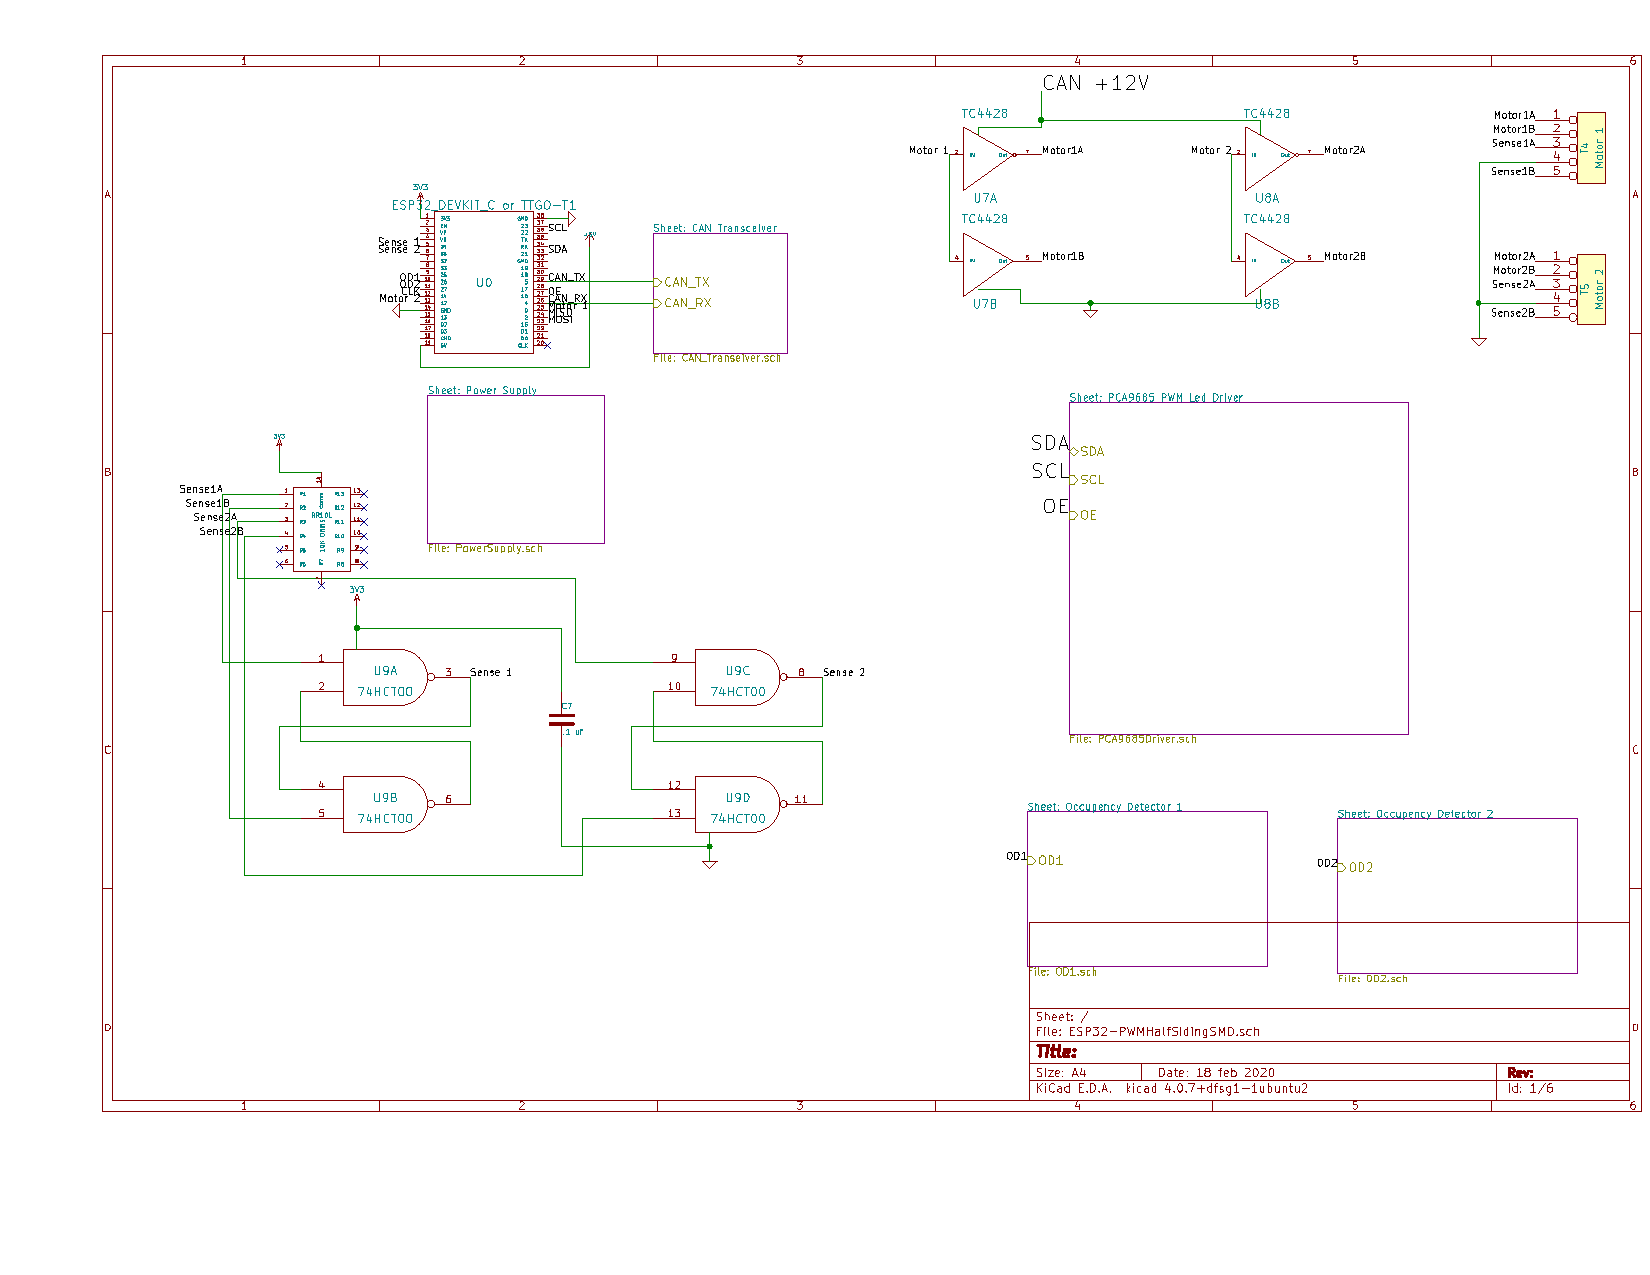
\includegraphics[width=5in]{ESP32-PWMHalfSidingSMD-1.pdf}
\caption{Circuit Diagram of the ESP32-PWMHalfSidingSMD, page 1 (ESP32 MCU and 
Turnout Driver and Sense)}
\end{centering}\end{figure}

The turnout control has two parts. There is an output section that contains
two TC4428 chips. Each chip has a non-inverting and an inverting driver. The
inputs of both drivers are connected to one of the motor GPIO pins. The output
are wired to the terminal block for a one of the motors. For any given logic
state of the motor control output, one of the drivers is ``on'' and the other
is ``off'', thus one motor terminal is ground and one is raised to the 12V
supply. This means alternative states of the logic line will drive the stall
motor in alternative directions. 

The other section is a pair of flip-flop debounce circuits, one for each of
two SPDT switch contacts that report the position of the turnout points. The
output of these flip-flops goes to a pair of GPIO input pins.

\clearpage
\subsection{CAN Transceiver}
\begin{figure}[hbpt]\begin{centering}%
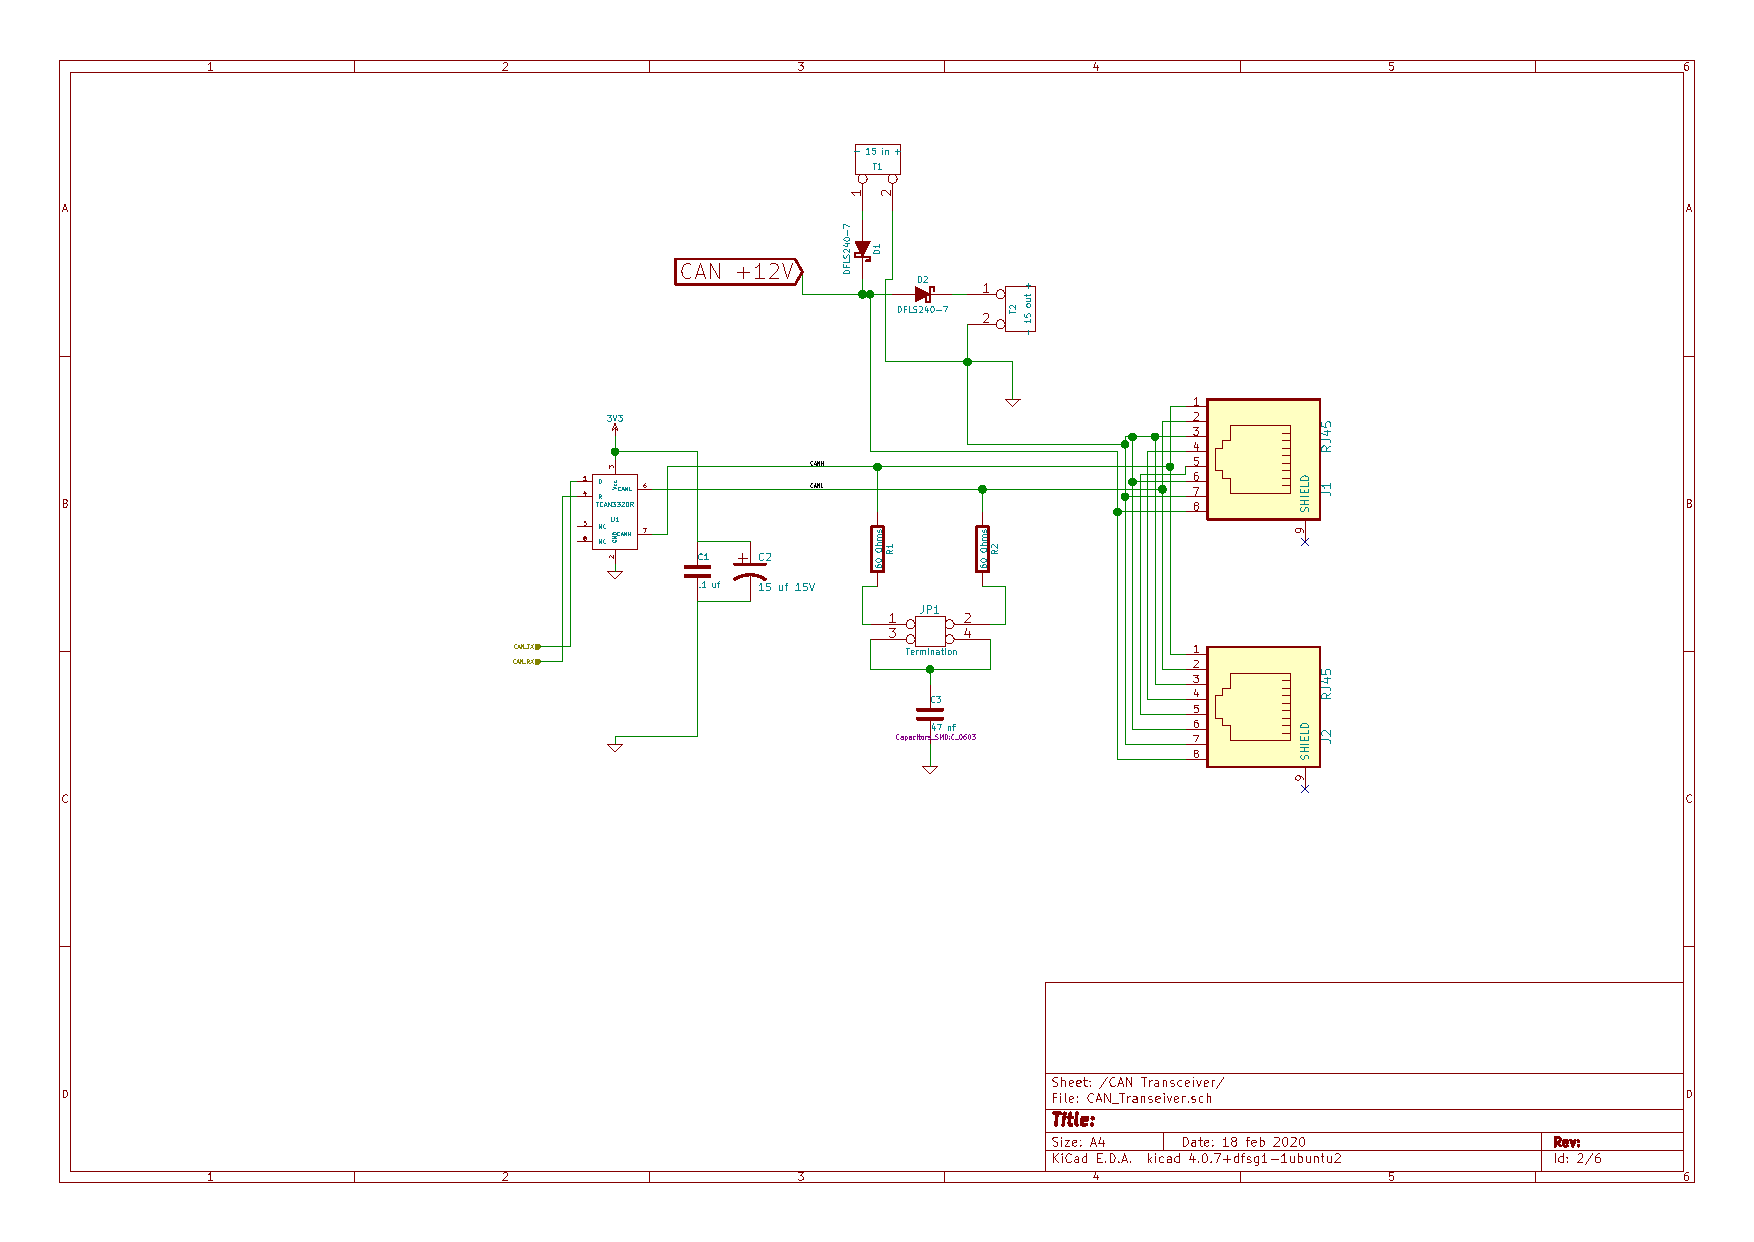
\includegraphics[width=5in]{ESP32-PWMHalfSidingSMD-2.pdf}
\caption{Circuit Diagram of the ESP32-PWMHalfSidingSMD, page 2 (CAN Transceiver)}
\end{centering}\end{figure}

This section contains the CAN Transceiver, along with a termination jumper 
block. Power insertion and pick off and the RJ45 Jacks.

\clearpage
\subsection{Power Supply}
\begin{figure}[hbpt]\begin{centering}%
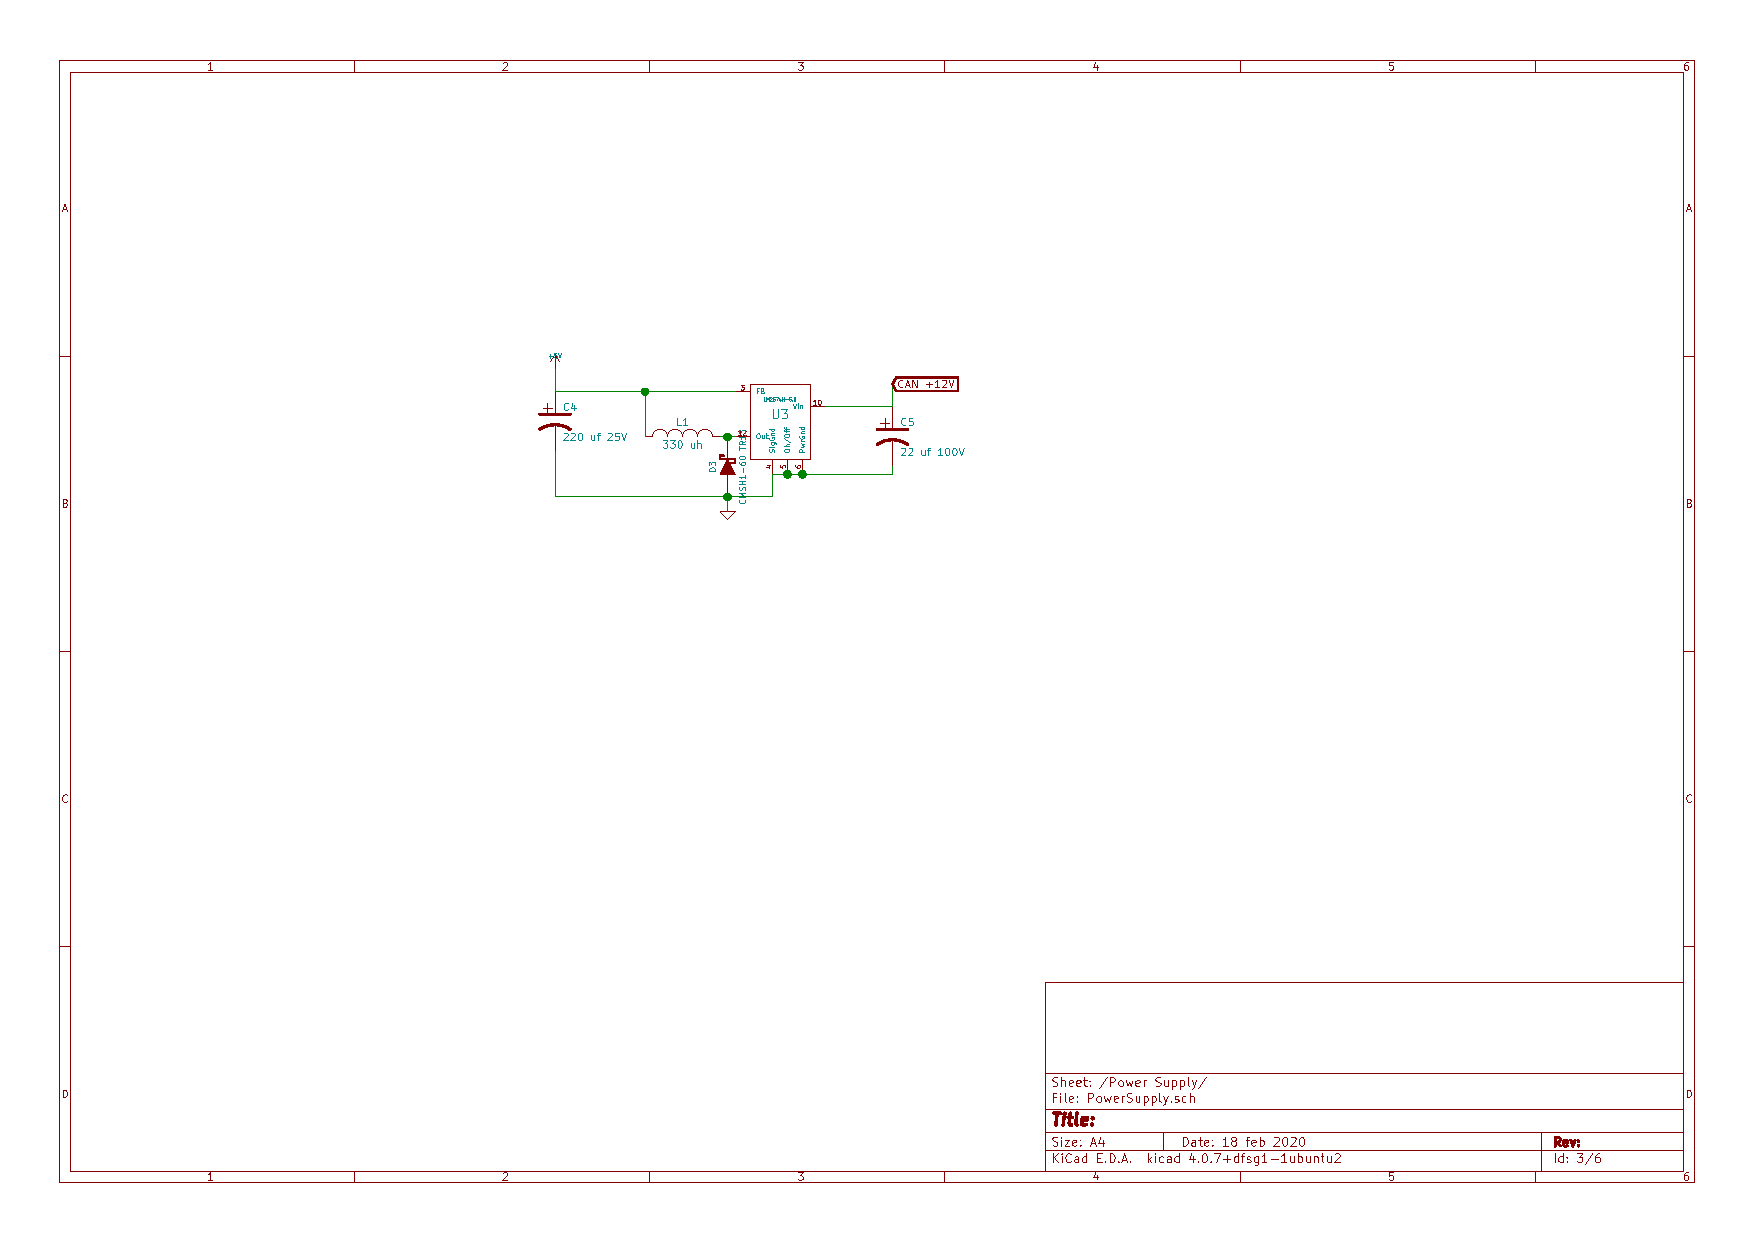
\includegraphics[width=5in]{ESP32-PWMHalfSidingSMD-3.pdf}
\caption{Circuit Diagram of the ESP32-PWMHalfSidingSMD, page 3 (Power Supply)}
\end{centering}\end{figure}

This section contains a 5V power supply that takes the nominal 12V on the CAN 
power bus and regulates it down to 5V to supply the ESP32 MCU board.

\clearpage
\subsection{Occupancy Detectors}
\begin{figure}[hbpt]\begin{centering}%
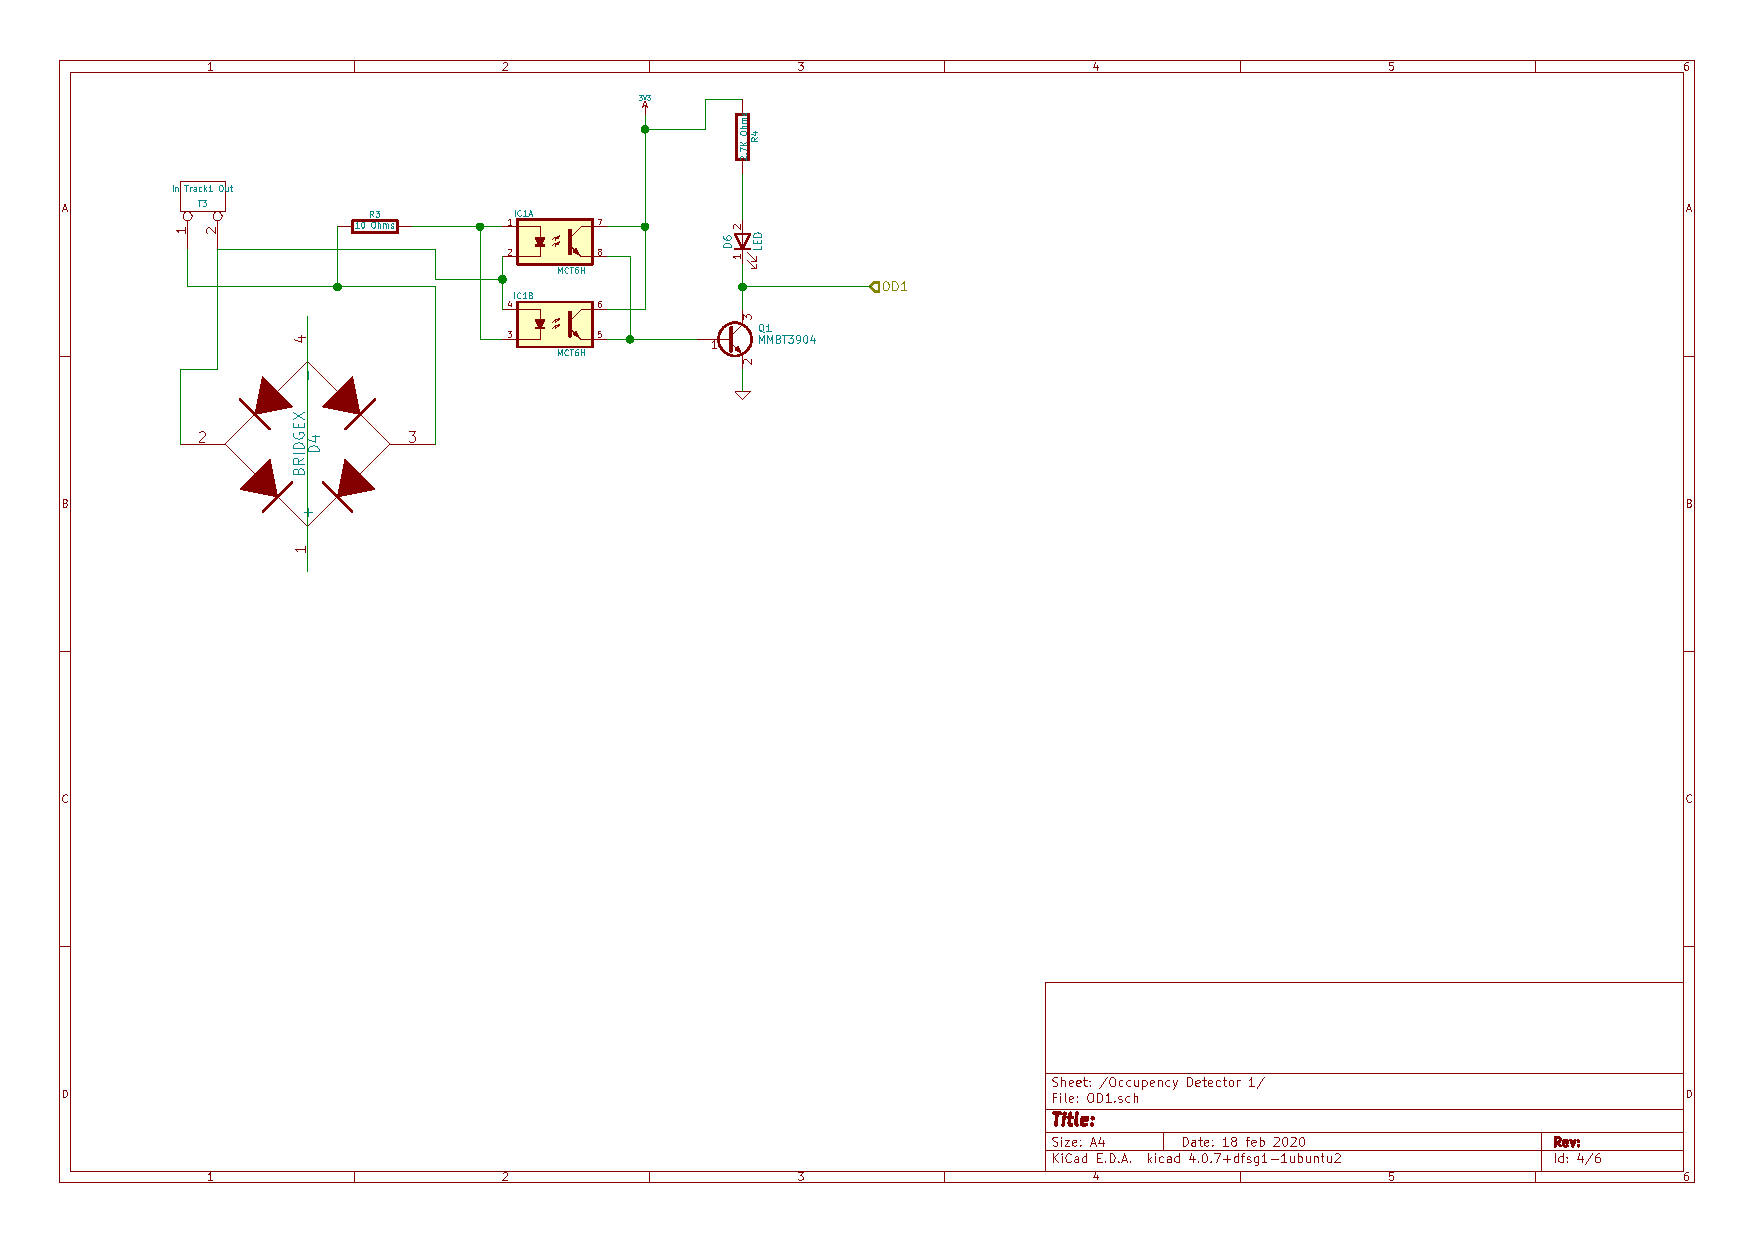
\includegraphics[width=5in]{ESP32-PWMHalfSidingSMD-4.pdf}
\caption{Circuit Diagram of the ESP32-PWMHalfSidingSMD, page 4 (Occupancy 
Detector 1)}
\end{centering}\end{figure}
\begin{figure}[hbpt]\begin{centering}%
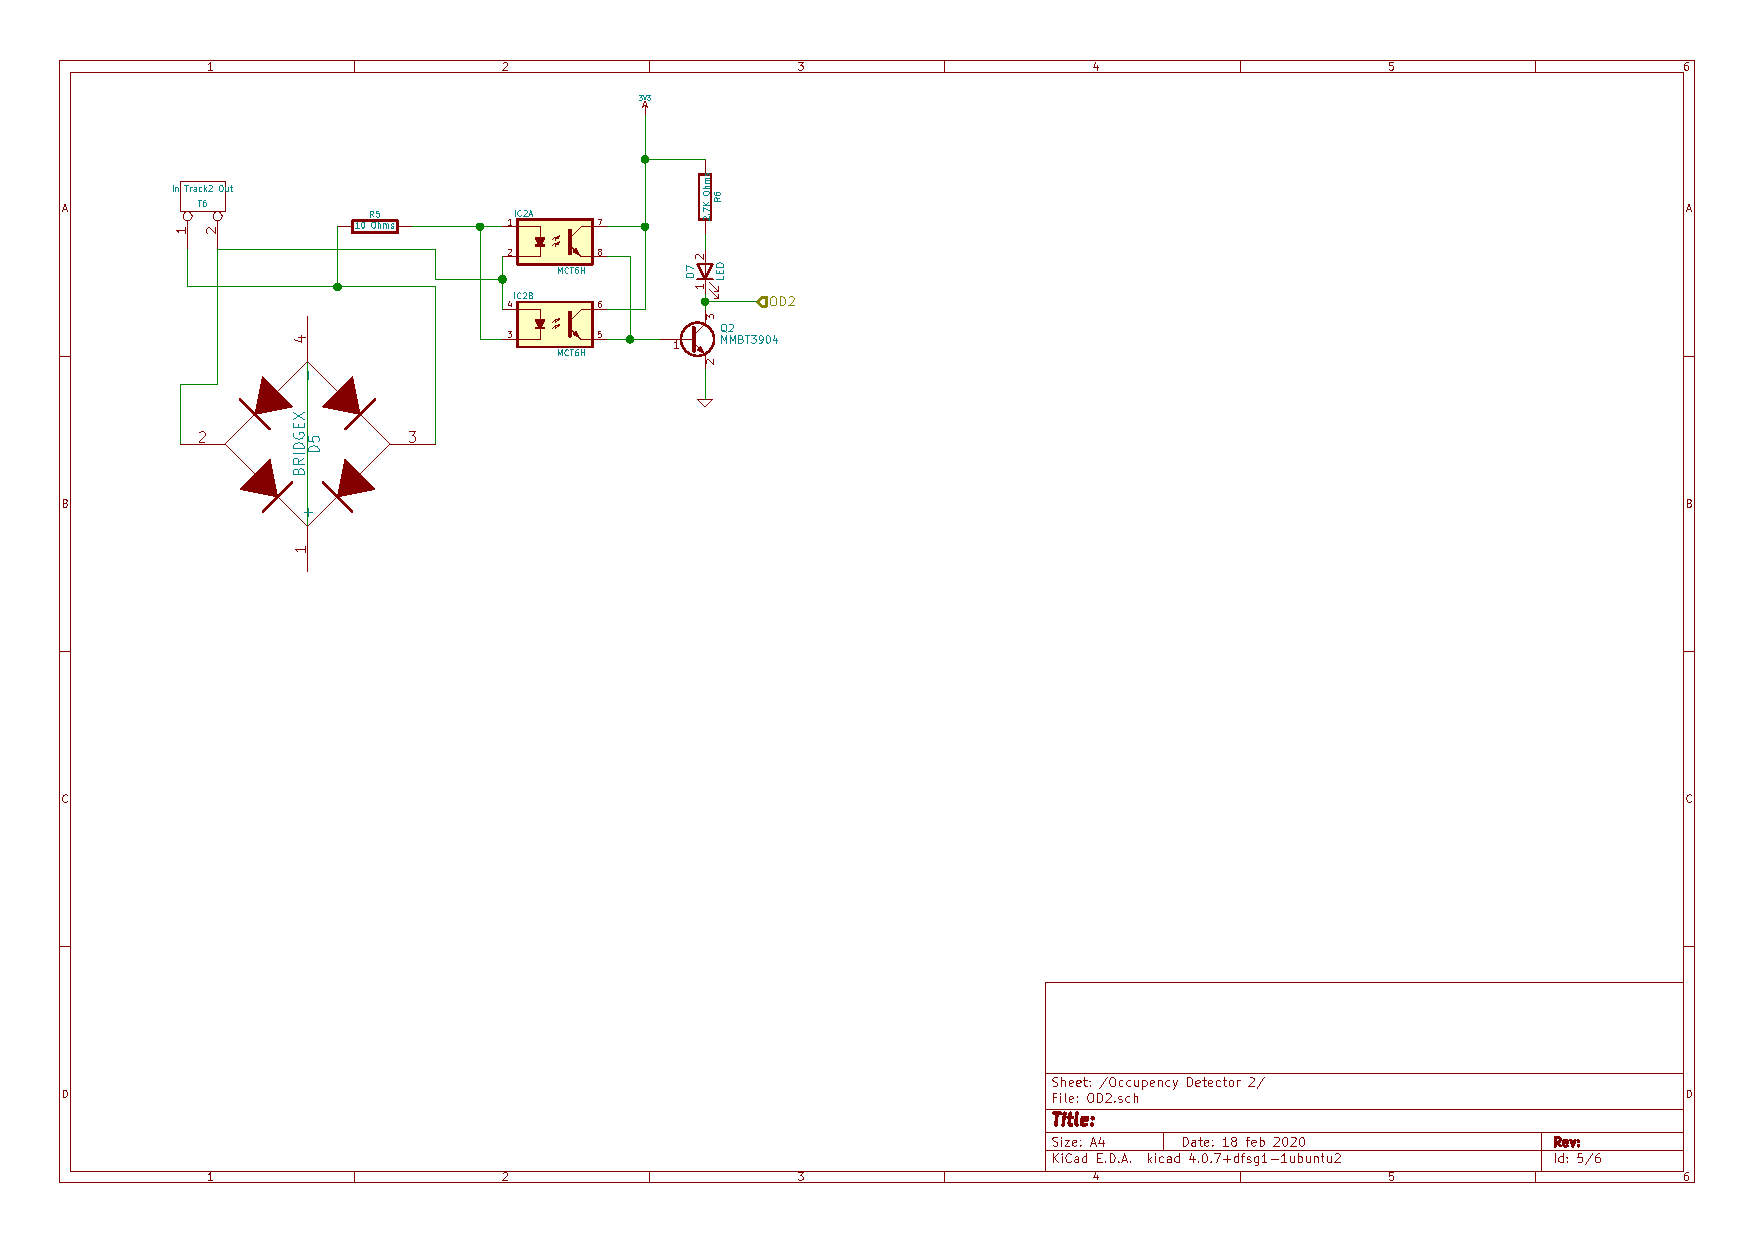
\includegraphics[width=5in]{ESP32-PWMHalfSidingSMD-5.pdf}
\caption{Circuit Diagram of the ESP32-PWMHalfSidingSMD, page 5 (Occupancy 
Detector 2)}
\end{centering}\end{figure}

The occupancy detectors use optoisolators in series with the track power 
supply.  There is a heavy duty bridge rectifier in parallel with the 
optoisolators to carry the bulk of the current to the track.  They will work 
with either DC or DCC track power.

\clearpage
\subsection{PWM LED Driver}
\begin{figure}[hbpt]\begin{centering}%
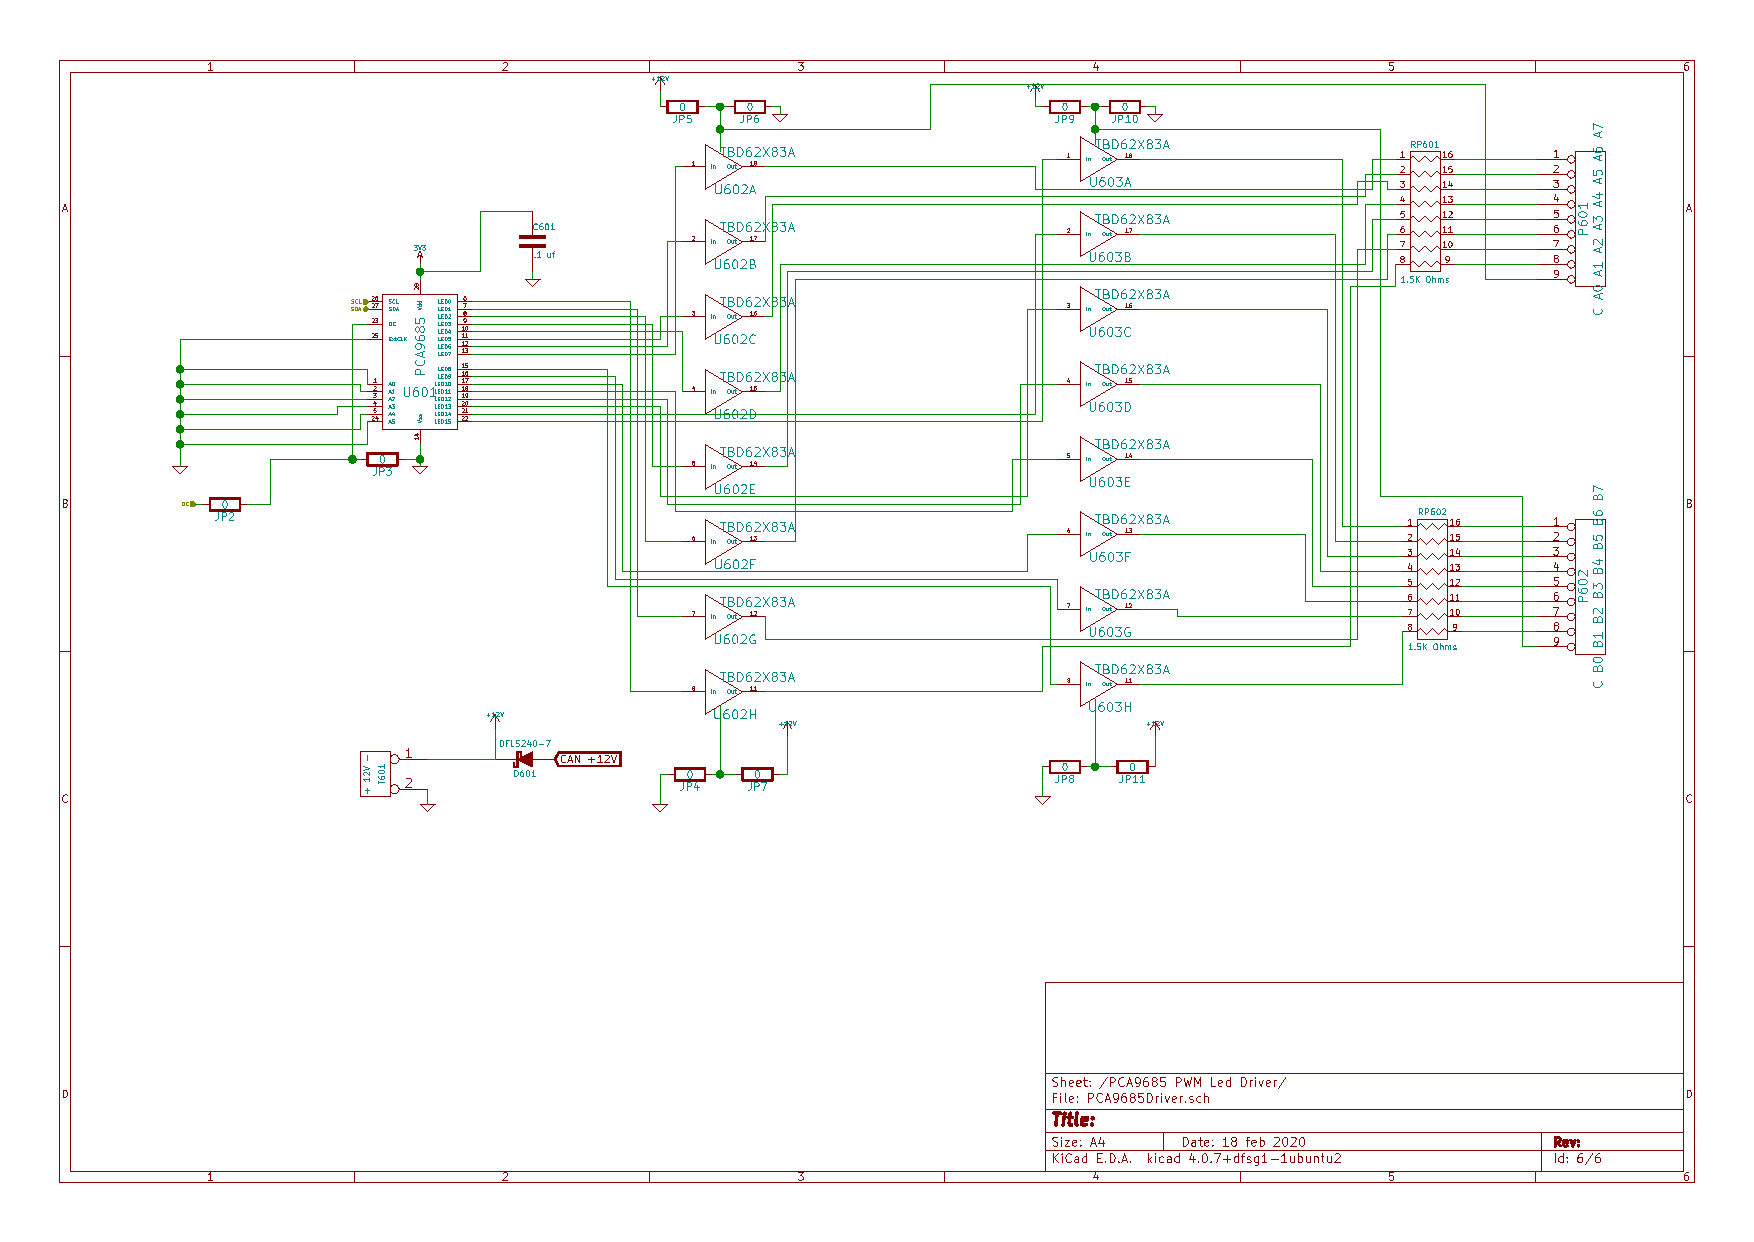
\includegraphics[width=5in]{ESP32-PWMHalfSidingSMD-6.pdf}
\caption{Circuit Diagram of the ESP32-PWMHalfSidingSMD, page 6 (PWM LED Driver)}
\end{centering}\end{figure}

The PWM LED Driver uses a PCA9685 which is a 16 channel, 12 bit PWD LED 
driver.  A pair of octal MOSFET drivers and series load resistors are also 
included on the board.  The MOSFET drivers come in both inverting (low-side 
drive) and non-inverting (high-side drive), so it is possible to support both 
common anode and common cathode LED signals.

\clearpage
\section{User Installed Parts}

\begin{centering}\begin{tabular}{|r|l|l|p{1.5in}|p{1.5in}|}
\hline
Index&Qty&Refs&Mouser Part Number&Description\\   
\hline
1&2&J1, J2&710-615008144221&RJ45 Jacks\\
\hline
2&1&JP1&649-67997-404HLF&Termination Jumper -- 2x2 pin header\\
\hline
3&1&J3&649-1012937890304BLF&I2C SCL Select Jumper -- 3-pos 2.54 pitch pin header\\
\hline
4&2&P601, P602&651-1725724&Signal Lamp Terminals -- 9-pos 2.54 pitch screw terminals\\
\hline
5&3&T1, T2, T601&651-1725656&LCC and Signal power -- 2-pos 2.54 pitch screw terminals\\
\hline
6&2&T3, T6&490-TB007-508-02BE&Occupancy Terminals -- 2-pos 5.08 pitch screw terminals\\
\hline
7&2&T4, T5&651-1725685&Turnout terminals -- 5-pos 2.54 pitch screw terminals\\
\hline
8&2&U0&517-929974-01-19-RK&MCU Headers -- 19x1 pin socket headers\\
\hline
9&1&U0&517-929850-01-18-10&MCU Headers -- 18x1 pin socket headers\\
\hline
\end{tabular}\end{centering}

\section{Circuit Board Layout}
\begin{figure}[hbpt]\begin{centering}%
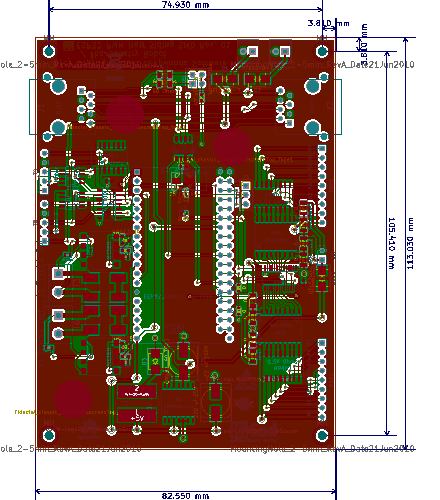
\includegraphics[width=5in]{ESP32-PWMHalfSidingSMD-brd.png}
\caption{Fabrication image of the ESP32-PWMHalfSiding board}
\end{centering}\end{figure}
\begin{figure}[hbpt]\begin{centering}%
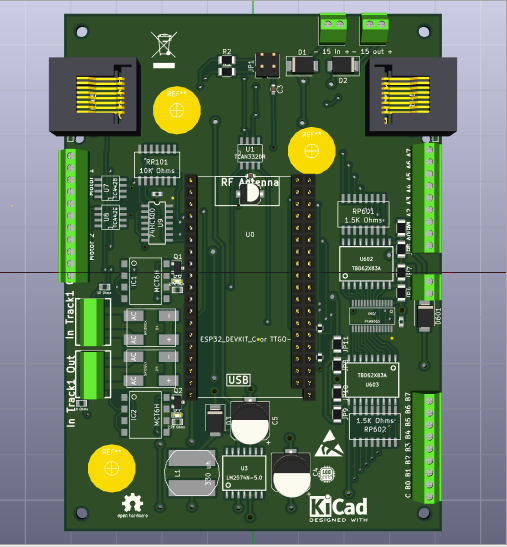
\includegraphics[width=5in]{ESP32-PWMHalfSidingSMD-top3D.png}
\caption{3D image of the ESP32-PWMHalfSiding board}
\end{centering}\end{figure}

\subsection{Notes on Building the board}
\begin{figure}[hbpt]\begin{centering}%
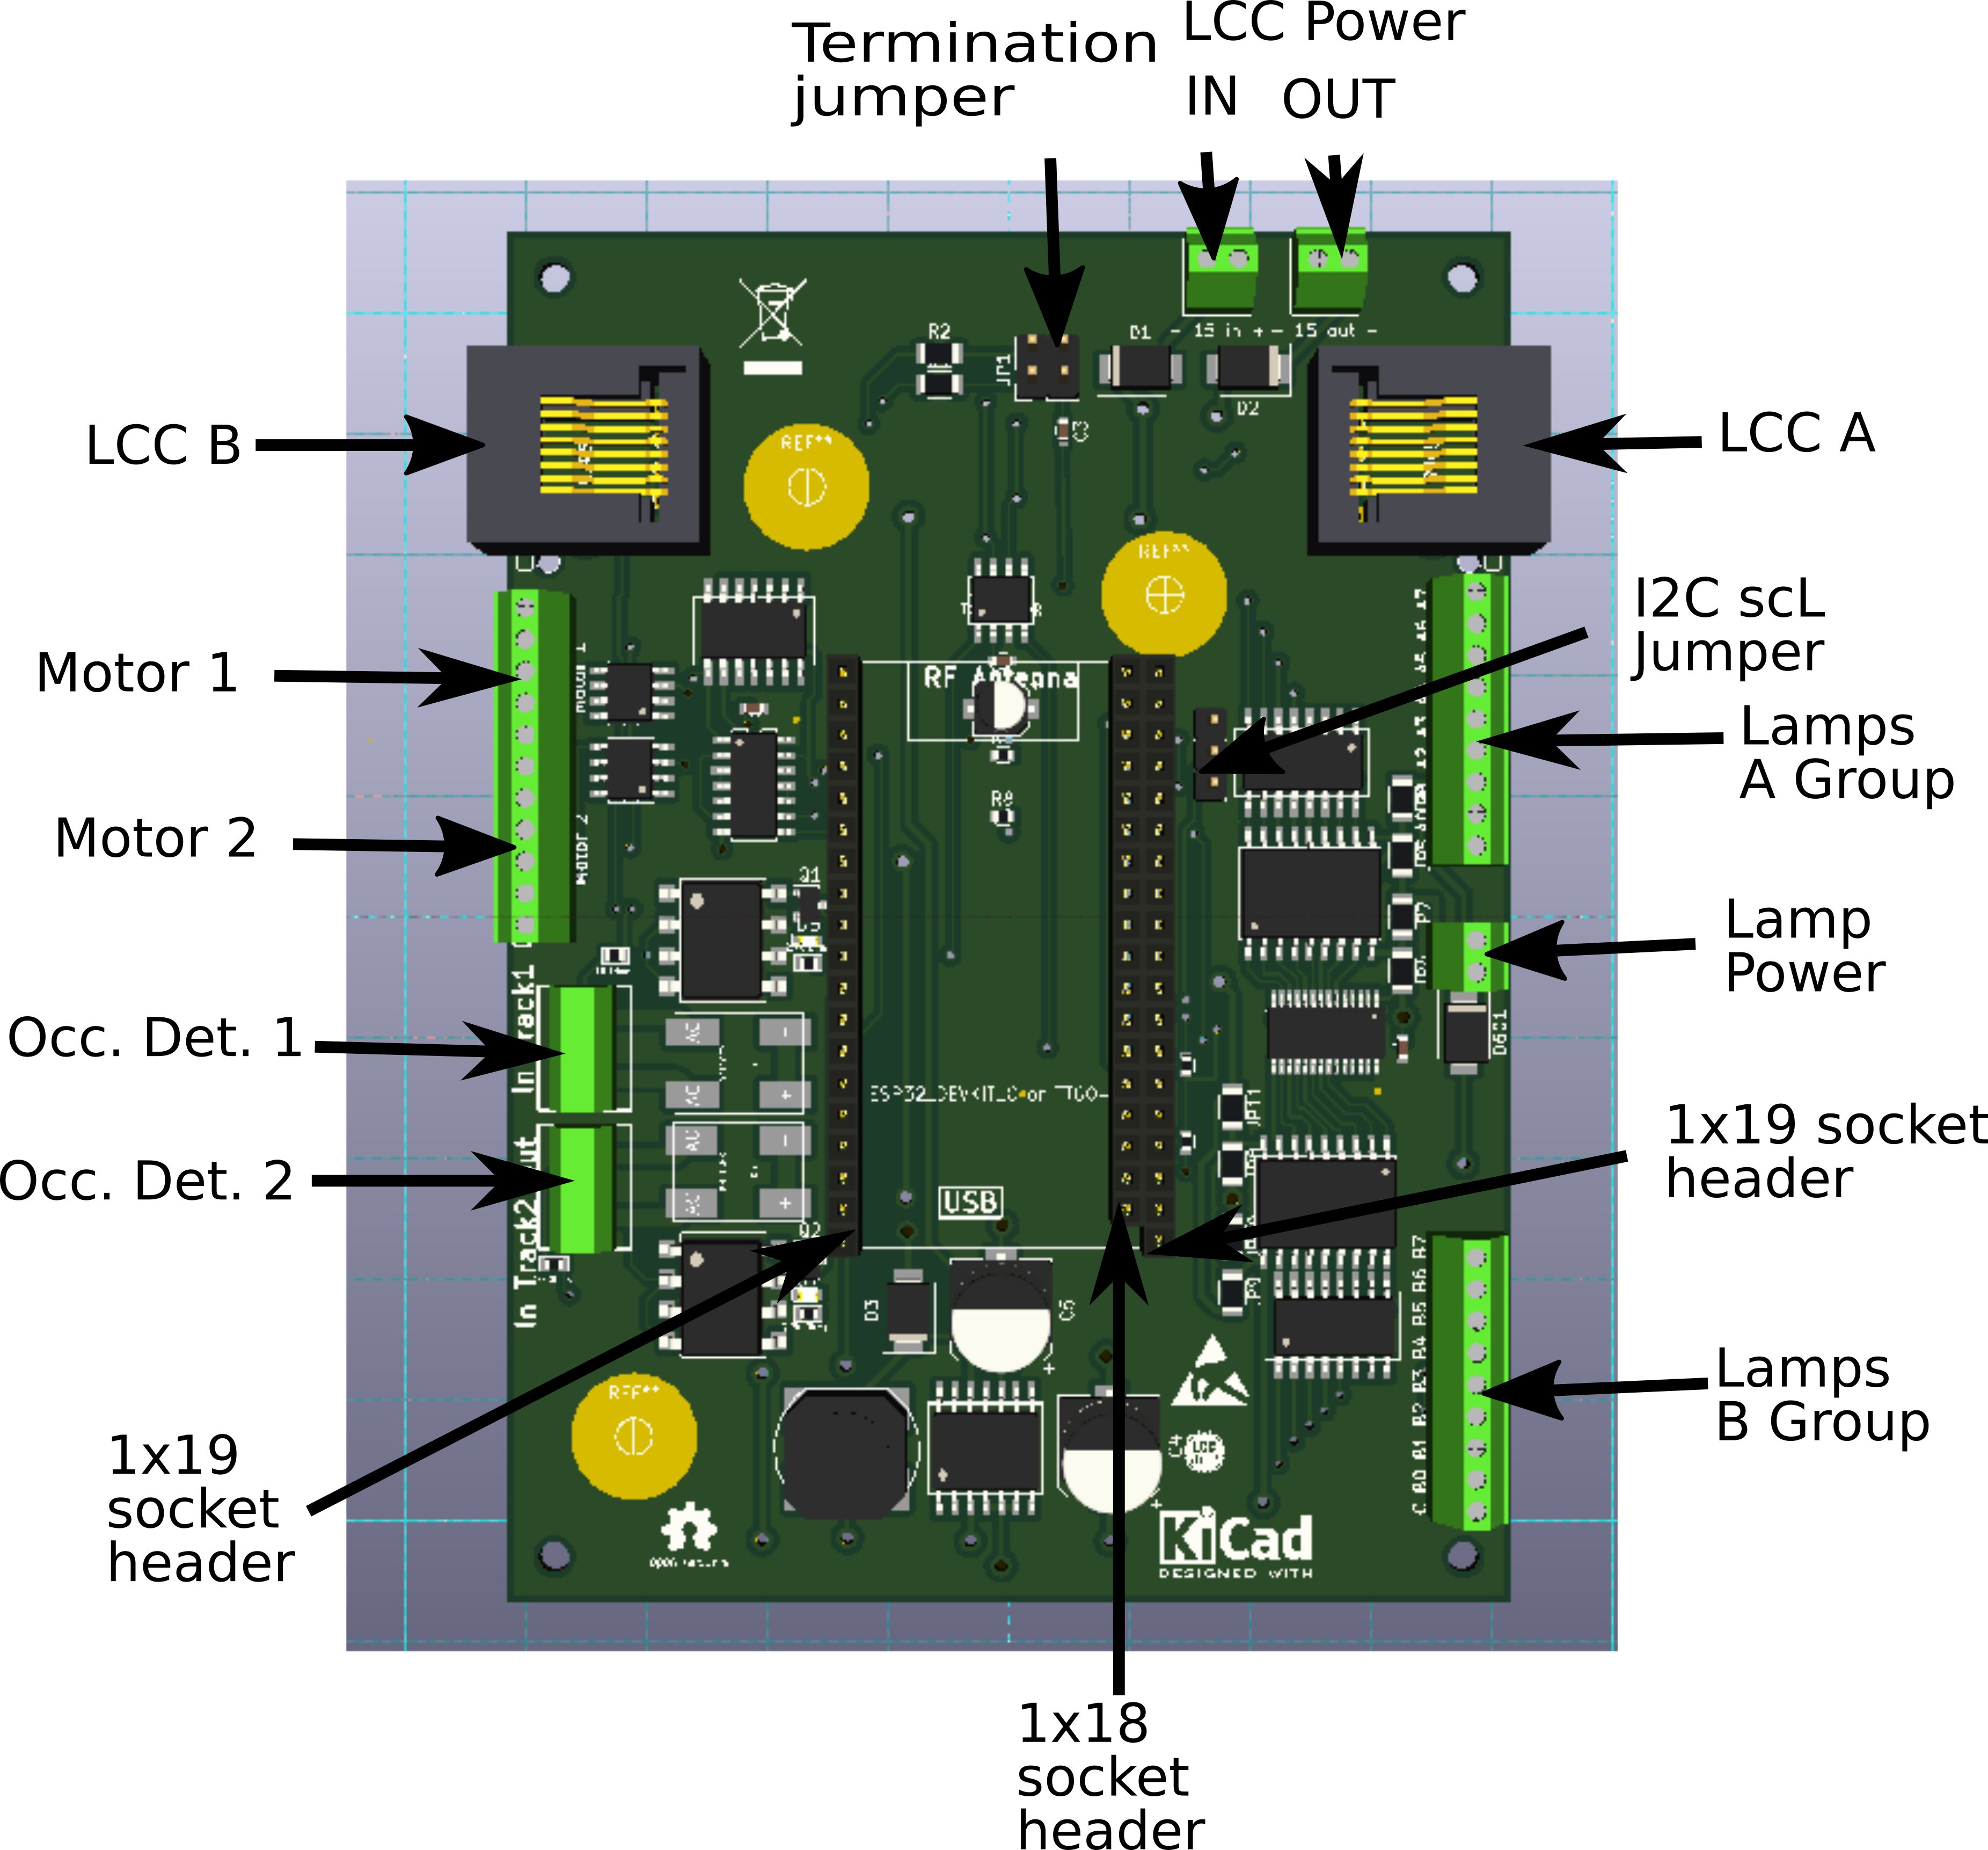
\includegraphics[width=5in]{ESP32HalfSidingWiringSMD.png}
\caption{Placement of terminal blocks, connectors, and jumper blocks.}
\end{centering}\end{figure}

The board comes with all the surface mount devices soldered to the board.  All 
you need to do is solder the through-hole parts, which consists of:

\begin{description}
\item[Screw Terminals] 3 2-position 2.54 pitch terminals (LCC power in and
out, lamp power in), 2 5-position 2.54 pitch terminals (motor 1 and motor
2), 2 9-position 2.54 pitch terminals (signal lamp outputs), and 2 2-position
5.08 pitch terminals (Occ. Det. 1 and Occ. Det. 2). 
\item[Pin Headers] 1 2x2 pin header (termination jumpers) and 1 1x3 pin header
(I2C SCL GPIO selection).
\item[Connectors] 2 RJ45 connectors (LCC Network).
\item[Pin Socket Headers] 2 19x1 and 1 18x1, for the MCU module.
\end{description}

For most of these parts you should solder one pin and then while pressing the
part against the board, reflow the solder to make sure the part is tight and
square to the board before letting the solder cool while holding the part
tight to the board. Before soldering the rest of the pins, check that the part
is fully tight and flush to the board. Also for the screw terminals, make sure
the wire openings are facing out from the board. The install ordering is from
shortest to tallest parts.

\clearpage
\section{Downloadables and Software Support}

The ESP32 needs to have a program installed in it to run the board.  This 
program can be downloaded from GitHub as part of the RRCircuits package: 
\url{https://github.com/RobertPHeller/RPi-RRCircuits}. The sketch is in the 
ESP32MRNSketches folder and is named ESP32-PWMHalfSiding. 


\subsection{Building and installing the software}


The ESP32 MCU is programmed with the Arduino IDE. It uses two libraries: the
FaBo PWM PCA9685 library for the PCA9685 chip and the OpenMRN\_lite library to
implement the OpenLCB/LCC stack. First you need to install board support for
the ESP32 and then install the FaBo PWM PCA9685 library. Both of these can be
done using the Arduino IDE board and library managers. Installing the
OpenMRN\_lite library is a little different. The OpenMRN\_lite library is part
of the OpenMRN package, available on GitHub here:
\url{https://github.com/bakerstu/openmrn}. You will also need the sketch for
this board which is also on GitHub in the RRCircuits repository:
\url{https://github.com/RobertPHeller/RPi-RRCircuits} in the
ESP32MRNSketches/ESP32-PWMHalfSiding. The kit includes a thumb drive that
contains two Zip files: one for the OpenMRN\_lite library
(\texttt{OpenMRN\_lite.zip}) and one for the sketch
(\texttt{ESP32-PWMHalfSiding.zip}). Just unpack the \texttt{OpenMRN\_lite.zip}
file under your Arduino libraries folder (usually named libraries in the
Arduino folder in your home folder). And then unpack the sketch
(\texttt{ESP32-PWMHalfSiding.zip}) directly under your Arduino folder. Then
open the sketch with the Arduino IDE. Before you compile it, you will need to
edit the NODEID.h file to set the node ID, which should be one of the node ids
you got from the OpenLCB website. If you have more than one of these boards,
you need to give each one a different node id.

Once you have built the sketch, you can upload it using an USB cable connected 
between your computer and the MCU board.

\subsection{Program Description}

The program consists of a main sketch file, and several support files.  Most 
of the support files implement I/O or logic elements:

\begin{description}
\item[Blink.h] This file provides support for blinking (flashing) signal 
lamps.
\item[config.h] This file defines the structure of the node's configuration.
\item[Lamp.h] This file implements the output functions for signal lamps.
\item[Logic.cpp, Logic.h] These files implement the Logic elements available 
in the node.
\item[Mast.cpp, Mast.h] These files implement signal masts.
\item[NODEID.h] This file contains the Node ID.
\item[OccupancyDetector.h] This file implements the occupancy detector inputs.
\item[Points.h] This file implements the point sense inputs.
\item[PWM.h] This file implements the PWM abstraction.
\item[Rule.cpp, Rule.h] These files implement traffic rules.
\item[TrackCircuit.cpp, TrackCircuit.h] These files implement track circuits.
\item[Turnout.h] This file implements the switch motor outputs.
\end{description}

\section{General Wiring Notes}

There are various terminal blocks, connectors, and jumper blocks on this
board. At the top end of the board are a pair of two position terminal blocks, 
one for injecting power into the LCC bus and one for extracting power from the 
LCC bus.  Between these terminal blocks is the termination jumper block for 
the LCC bus.  Below the LCC  power terminal blocks is a pair of RJ45 
connectors. These are for connecting the board to the LCC bus.  These 
connectors are wired in parallel.  Down along the left side are the two stall 
motor terminal blocks (small 5 position terminal blocks) and the occupancy 
detector terminal blocks (large 2 position terminal blocks).  On the right 
side are two 9 position terminal blocks for the signal lamp LEDs.  Finally, at 
the bottom right is a two position terminal block to (optionally) provide 
power for the signal lamp LEDs.

\subsection{LCC Power}

Power can be optionally injected into the LCC bus or extracted from the LCC 
bus. Power can be injected to into the LCC bus to power this and other boards. 
Power can also be extracted to power local devices.

\subsection{I2C SCL GPIO Selection}

\begin{figure}[hbpt]\begin{centering}%
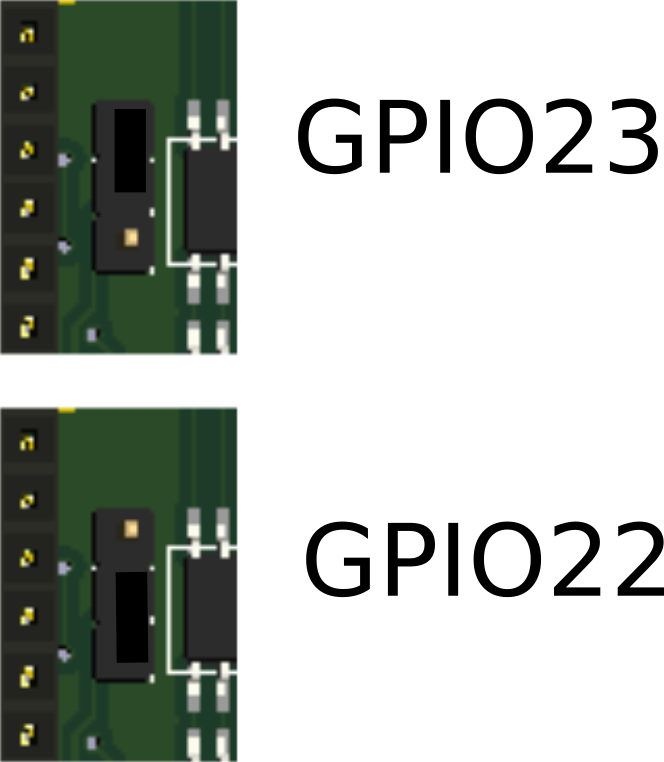
\includegraphics{I2C-SCL-Jumper_edited.png}
\caption{I2C SCL Jumper Options}
\label{fig:ESP32-PWMHalfSidingI2CSCLJumper}
\end{centering}\end{figure}
There is a jumper to selecting the GPIO pin to use for I2C SCL line.  If you 
are using an ESP32 DevKit you would use GPIO 22.  If you are using a Lily Go 
TTGO-T1, you might want to use GPIO 23 since GPIO 22 on the TTGO-T1 is wired 
to its on-board LED and this has been known to cause issues with the I2C 
interface.  If you select Arduino IDE's board type ``TTGO-T1'', SCL is mapped 
to GPIO 23 -- it is possible to select the generic ESP32 DevKit as the board 
type to compile for the ``TTGO-T1'', in which case SCL is mapped to GPIO 22.  
You should install a shunt jumper that matches how you compiled the firmware.

\subsection{LCC Bus connections and termination}

\begin{figure}[hbpt]\begin{centering}%
\includegraphics{ESP32-PWMHalfSidingTermination.png}
\caption{Termination Jumper Options}
\label{fig:ESP32-PWMHalfSidingTermination}
\end{centering}\end{figure}
The two RJ45 connections connect to the LCC bus.  If this board is at the end 
of bus, you will need to terminate the bus.  There are two possible 
termination options as shown in 
Figure~\ref{fig:ESP32-PWMHalfSidingTermination}.

\subsection{Stall Motor connections}

\begin{figure}[hbpt]\begin{centering}%
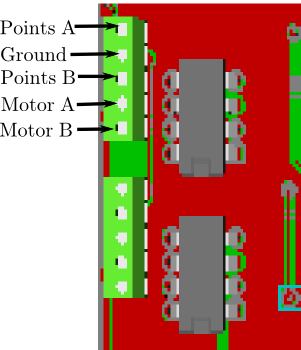
\includegraphics{ESP32-PWMHalfSidingTurnoutMotorsFig.png}
\caption{Stall Motor terminal block connections}
\label{fig:ESP32-PWMHalfSidingTurnoutMotorsFig}
\end{centering}\end{figure}
\begin{figure}[hbpt]\begin{centering}%
\includegraphics{ESP32-PWMHalfSidingTotoiseWiring.png}
\caption{Wiring a Tortoise to the ESP32-PWMHalfSiding Turnout Motors terminals}
\label{fig:ESP32-PWMHalfSidingTotoiseWiring}
\end{centering}\end{figure}
The five position Stall Motor terminal blocks, shown in 
Figure~\ref{fig:ESP32-PWMHalfSidingTurnoutMotorsFig}, connect to the turnout 
stall motors, the Motor A and Motor B connections go to the motor (pins 1 and 
8 of a tortoise), the other three connections go to a single pole double 
through switch contacts to sense the position of the stall motor / points. 
There are contacts available on tortoise stall motor that can be used for this 
purpose, as shown in Figure~\ref{fig:ESP32-PWMHalfSidingTotoiseWiring}.

\clearpage
\subsection{Occupancy Detector connections}

\begin{figure}[hbpt]\begin{centering}%
\includegraphics{ESP32-PWMHalfSidingOccupancyDetectors.png}
\caption{Occupancy Detector Wiring}
\label{fig:ESP32-PWMHalfSidingOccupancyDetectors}
\end{centering}\end{figure}
The larger two position Occupancy Detector terminal blocks are connected to 
the track power feeds as shown in 
Figure~\ref{fig:ESP32-PWMHalfSidingOccupancyDetectors}.

\clearpage
\subsection{Signal Lamp (LED) connections}

\begin{figure}[hbpt]\begin{centering}%
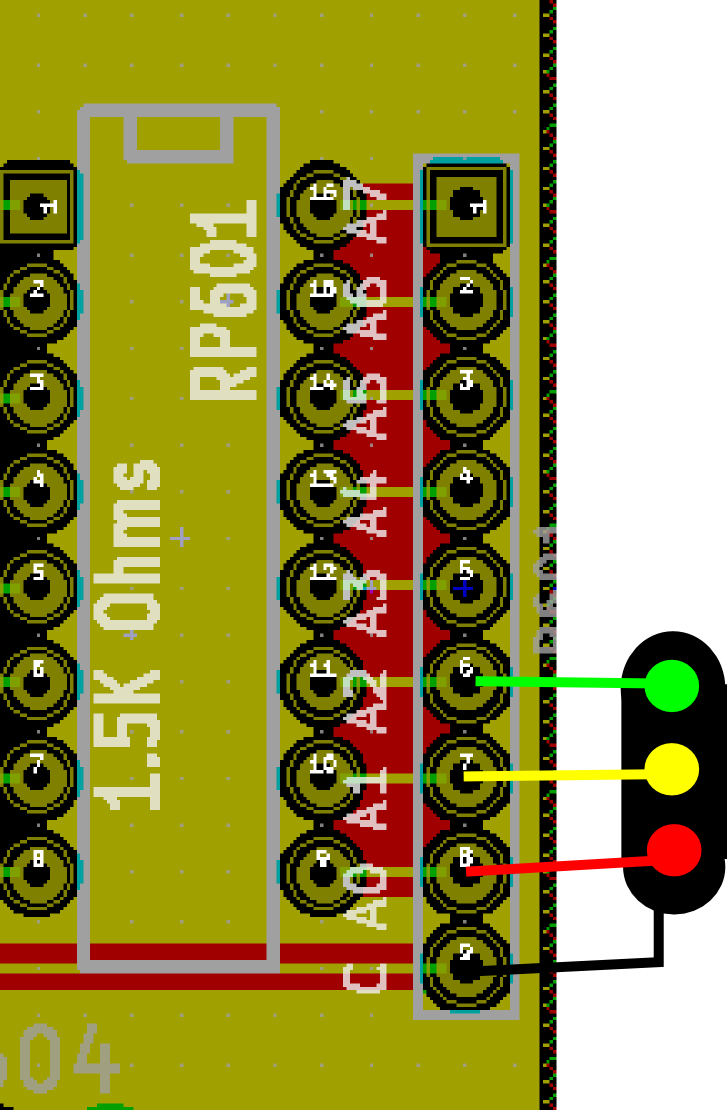
\includegraphics{ESP32-PWMHalfSidingLampDivers.png}
\caption{Typical Signal Lamp Diver Wiring}
\label{fig:ESP32-PWMHalfSidingLampDivers}
\end{centering}\end{figure}
Signal lamp diver wiring assumes common cathode or common anode signals as 
shown Figure~\ref{fig:ESP32-PWMHalfSidingLampDivers}.  

\clearpage
\section{Application Notes}

Three applications will presented, a typical siding using two boards, an 
implementation of a section of Automatic Block Signals, and Crossing with 
Interchange.  Other trackwork arrangements are possible as well.


\subsection{Typical Siding}

\begin{figure}[hbpt]\begin{centering}%
\includegraphics[width=5in]{ExampleSiding.png}
\caption{A Typical Siding}
\label{fig:ExampleSiding}
\end{centering}\end{figure}
\begin{figure}[hbpt]\begin{centering}%
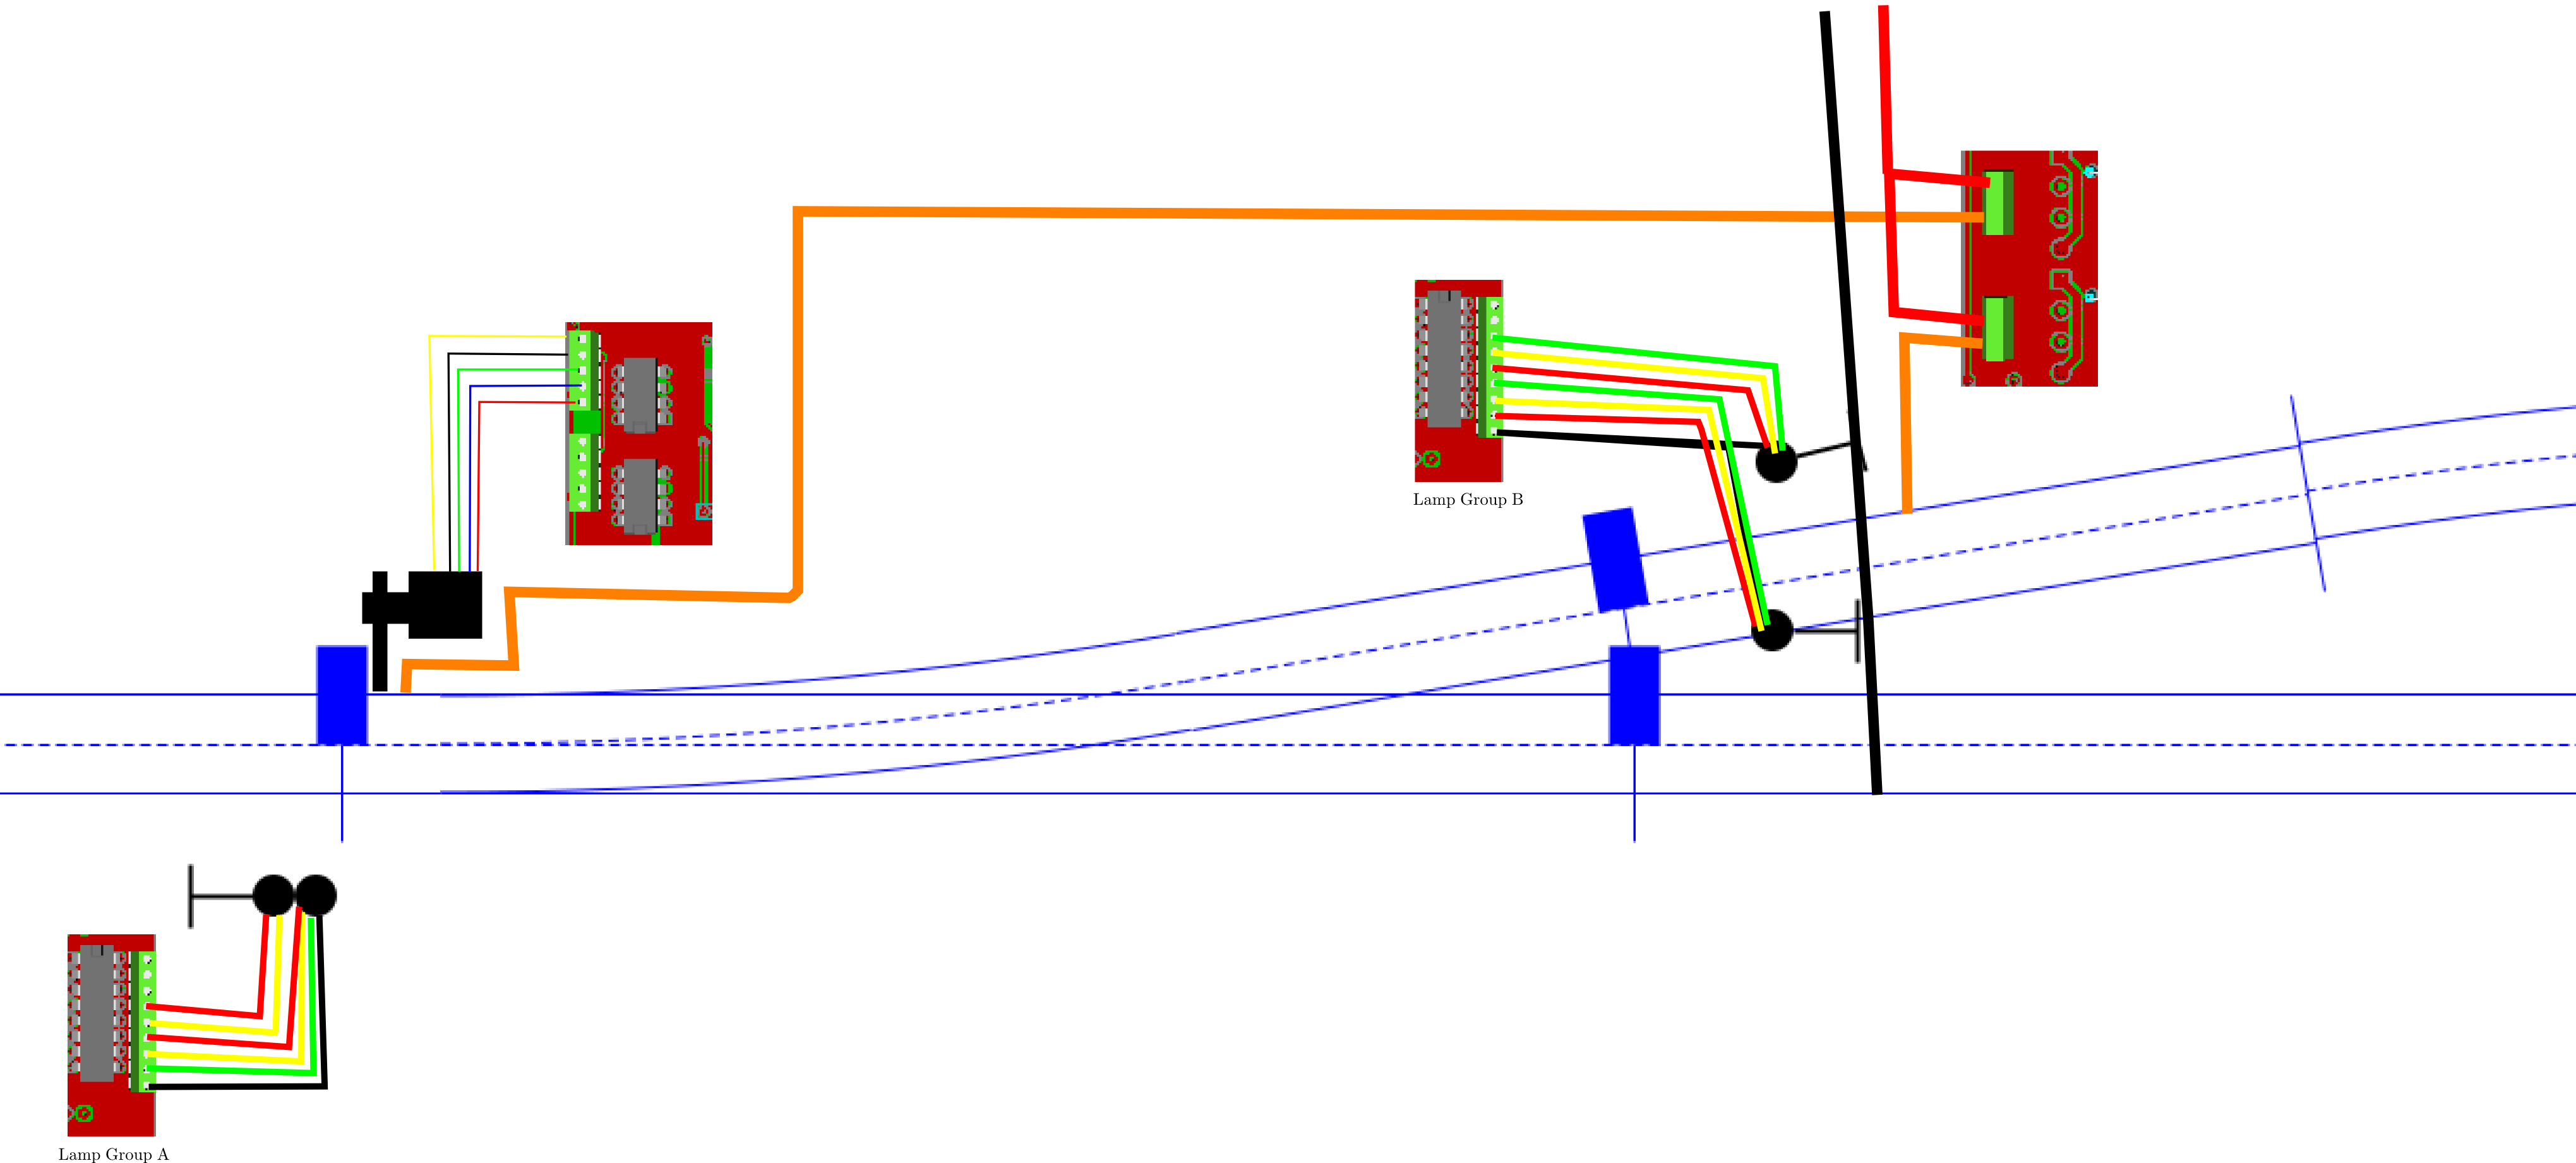
\includegraphics[width=5in]{ESP32HalfSiding-CP1Wiring.png}
\caption{Wiring the ESP32HalfSiding board to the control elements of CP1 (West 
end of the siding)}
\label{fig:ESP32HalfSiding-CP1Wiring}
\end{centering}\end{figure}
A typical siding is shown in Figure~\ref{fig:ExampleSiding}. And the wiring of 
the west end, CP1, is shown in Figure~\ref{fig:ESP32HalfSiding-CP1Wiring}. The 
other end is wired similarly (except that the second occupancy detector is 
wired to the main line block between the turnouts).

\subsubsection{Configuring the CP1 node (west end)}

\paragraph{Node identification configuration}
\begin{figure}[hbpt]\begin{centering}%
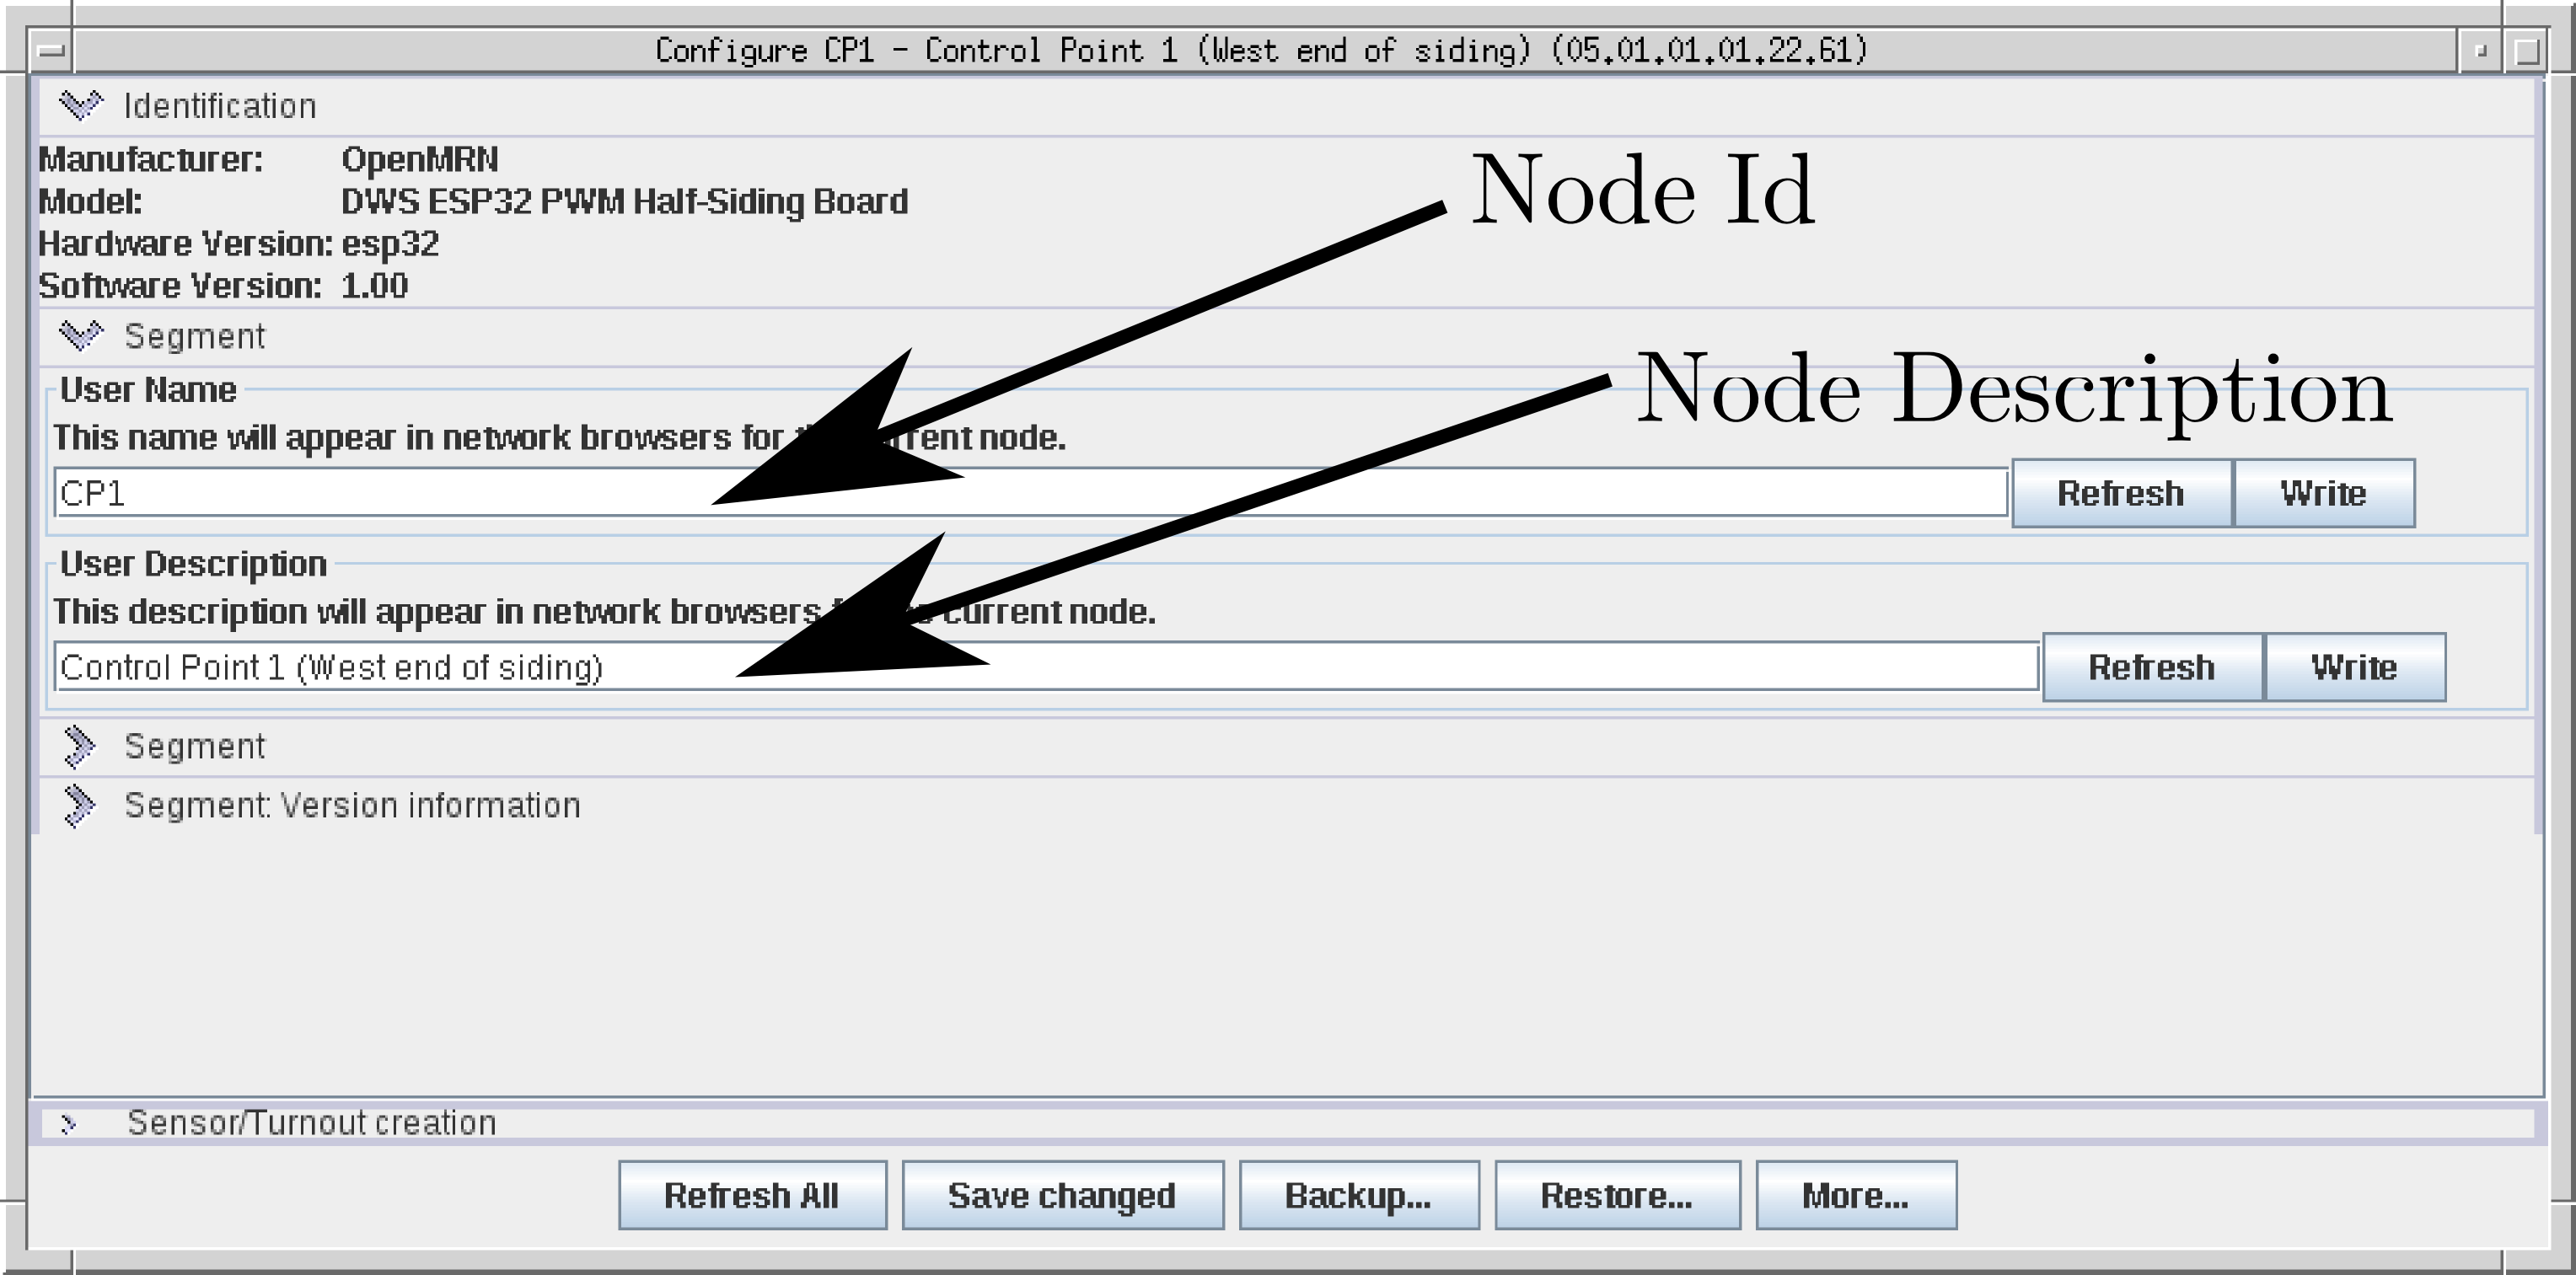
\includegraphics[width=5in]{CP1-ID-Config-Annotated.png}
\caption{CP1 Node ID configuration}
\label{fig:CP1-ID-Config}
\end{centering}\end{figure}
First the node's user name and description is configured.  This makes it easier 
to find the node in the node listing.

\clearpage
\paragraph{Occupancy Detector configuration}
\begin{figure}[hbpt]\begin{centering}%
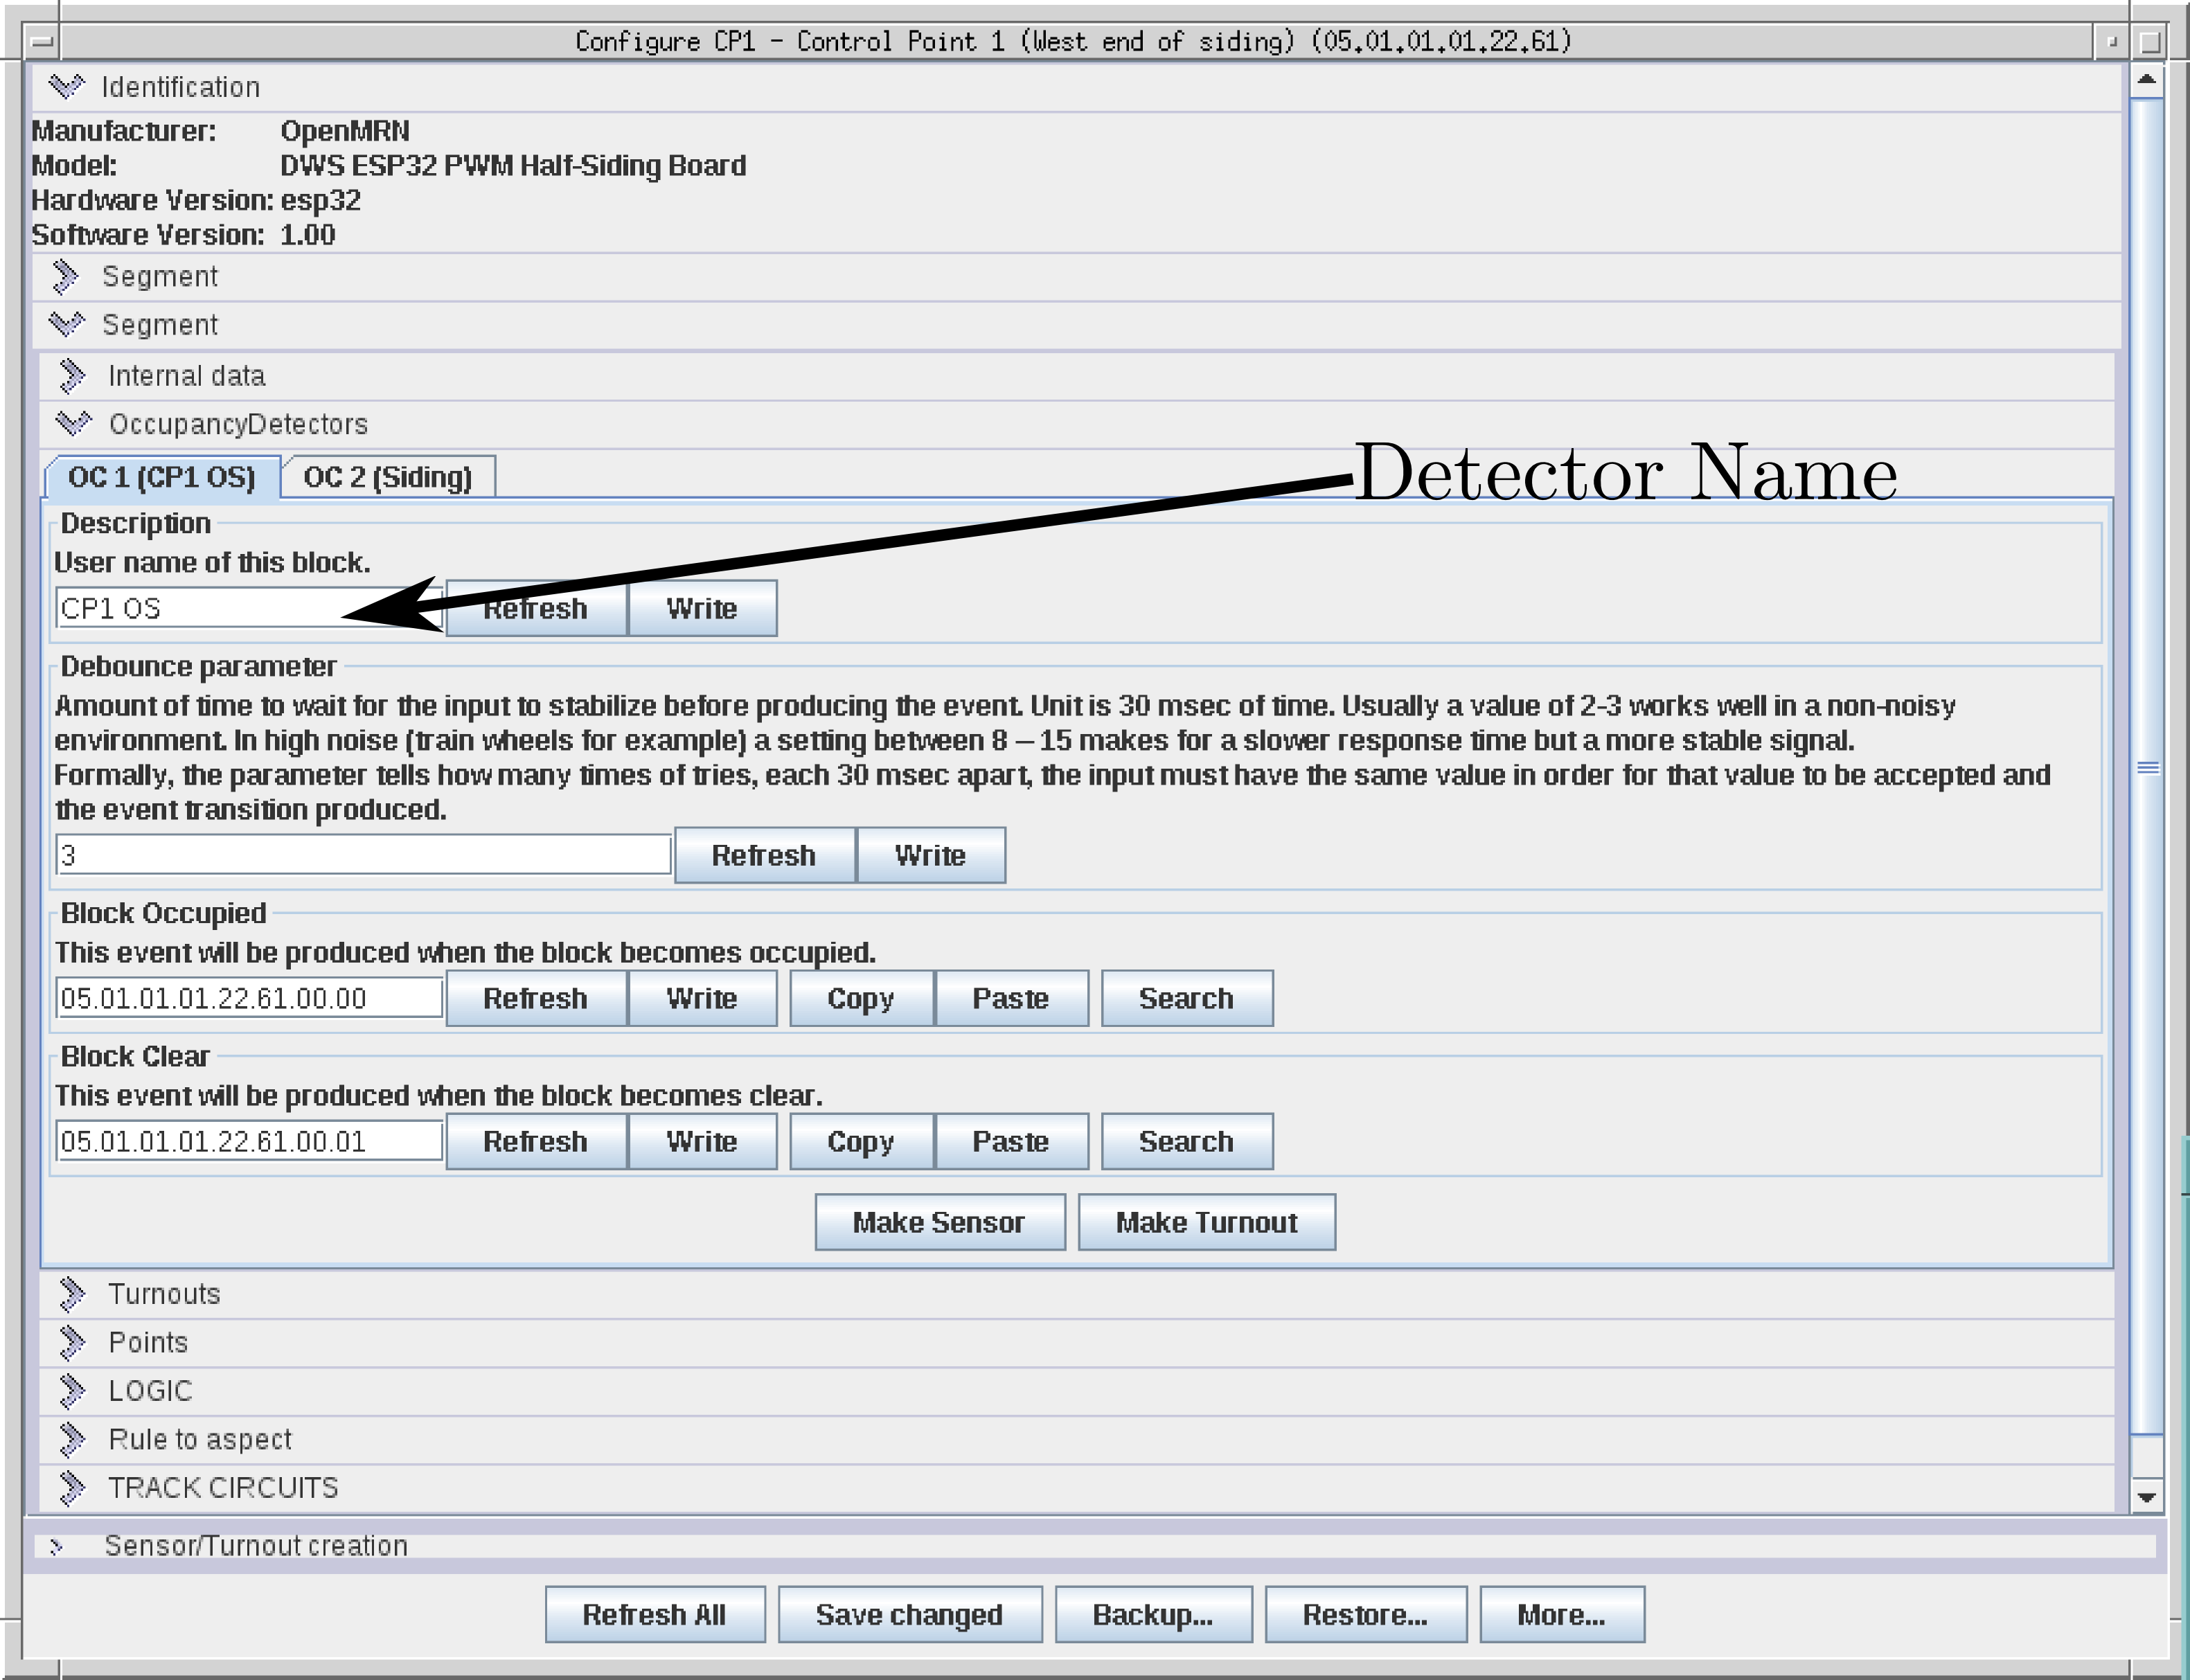
\includegraphics[width=5in]{CP1-OC-Config-Annotated.png}
\caption{CP1 Occupancy Detectors configuration}
\label{fig:CP1-OC-Config}
\end{centering}\end{figure}
Next we configure the Occupancy Detectors.  All we do at this point is fill in 
the names of the blocks.  This helps us when we grab the event ids later.
 
\clearpage
\paragraph{Turnout and Points configuration}
\begin{figure}[hbpt]\begin{centering}%
\includegraphics[width=5in]{CP1-Turnout-Config-Annotated.png}
\caption{CP1 Turnout and Points configuration}
\label{fig:CP1-Turnout-Config}
\end{centering}\end{figure}
Next we configure the Turnout and Points.  All we do at this point is fill in 
the name of the turnout.  We fill in the name for both the turnout and the 
points.  Only turnout 1 and points 1 are configured, since we are only using 
motor 1.

\clearpage
\paragraph{Signal mast configuration}
\begin{figure}[hbpt]\begin{centering}%
\includegraphics[width=5in]{CP1-Mast1-Config-Annotated.png}
\caption{CP1, Mast1 configuration}
\label{fig:CP1-Mast1-Config}
\end{centering}\end{figure}
Now we skip down to the masts. Mast 1 is the two head signal at the points
entrance, named CP1ME (Control Point 1, main, eastbound). We set its Mast ID
and copy and past its Track Circuit Link Address to Circuit 1. This is a 3
(green-yellow-red) over 2 (yellow-red) signal. It has 4 rules:
\begin{table}[htbp]\begin{centering}\begin{tabular}{|l|l|l|l|}
\hline
Tab&Rule Name&Track Speed&Appearance\\
\hline
Rule 1&0-Stop&Stop&Red over Red\\
Rule 2&21-Approach&Approach&Yellow over Red\\
Rule 3&29-Clear&Clear/Proceed&Green over Red\\
Rule 4&1-Take Siding&Slow&Red over Yellow\\
\hline
\end{tabular}
\caption{CP1ME's Rules}
\label{tab:CP1MERules}
\end{centering}\end{table}
The LEDs are wired to lamp group A as follows (see Figure~\ref{fig:ESP32HalfSiding-CP1Wiring}: 
\begin{description}
\item[A0] Upper Green
\item[A1] Upper Yellow
\item[A2] Upper Red
\item[A3] Lower Yellow
\item[A4] Lower Red
\end{description}
Lamp 1 will be the upper head and Lamp 2 will be for the lower head:
\begin{description}
\item[Rule 1: 0-Stop] Red over Red -- Lamp 1 will be A2 (upper red) and Lamp 2 
will be A4 (lower red).
\item[Rule 2: 21-Approach] Yellow over Red -- Lamp 1 will be A1 (upper yellow) 
and Lamp 2 will be A4 (lower red).
\item[Rule 3: 29-Clear] Green over Red -- Lamp 1 will be A0 (upper green) and 
Lamp 2 will be A4 (lower red).
\item[Rule 4: 1-Take Siding] Red over Yellow -- Lamp 1 will be A2 (upper red) 
and Lamp 2 will be A3 (lower yellow).
\end{description}

\clearpage
\paragraph{Logic block configuration}

\subparagraph{Logic for interlocking}
\begin{figure}[hbpt]\begin{centering}%                                         
\includegraphics[width=5in]{CP1-OSVeto-Normal1-Annotated.png}
\caption{CP1 OS Veto, part 1 (description, group function, variable 1)}
\label{fig:CP1-OSVeto-Normal1}
\end{centering}\end{figure}                                                    
\begin{figure}[hbpt]\begin{centering}%                                         
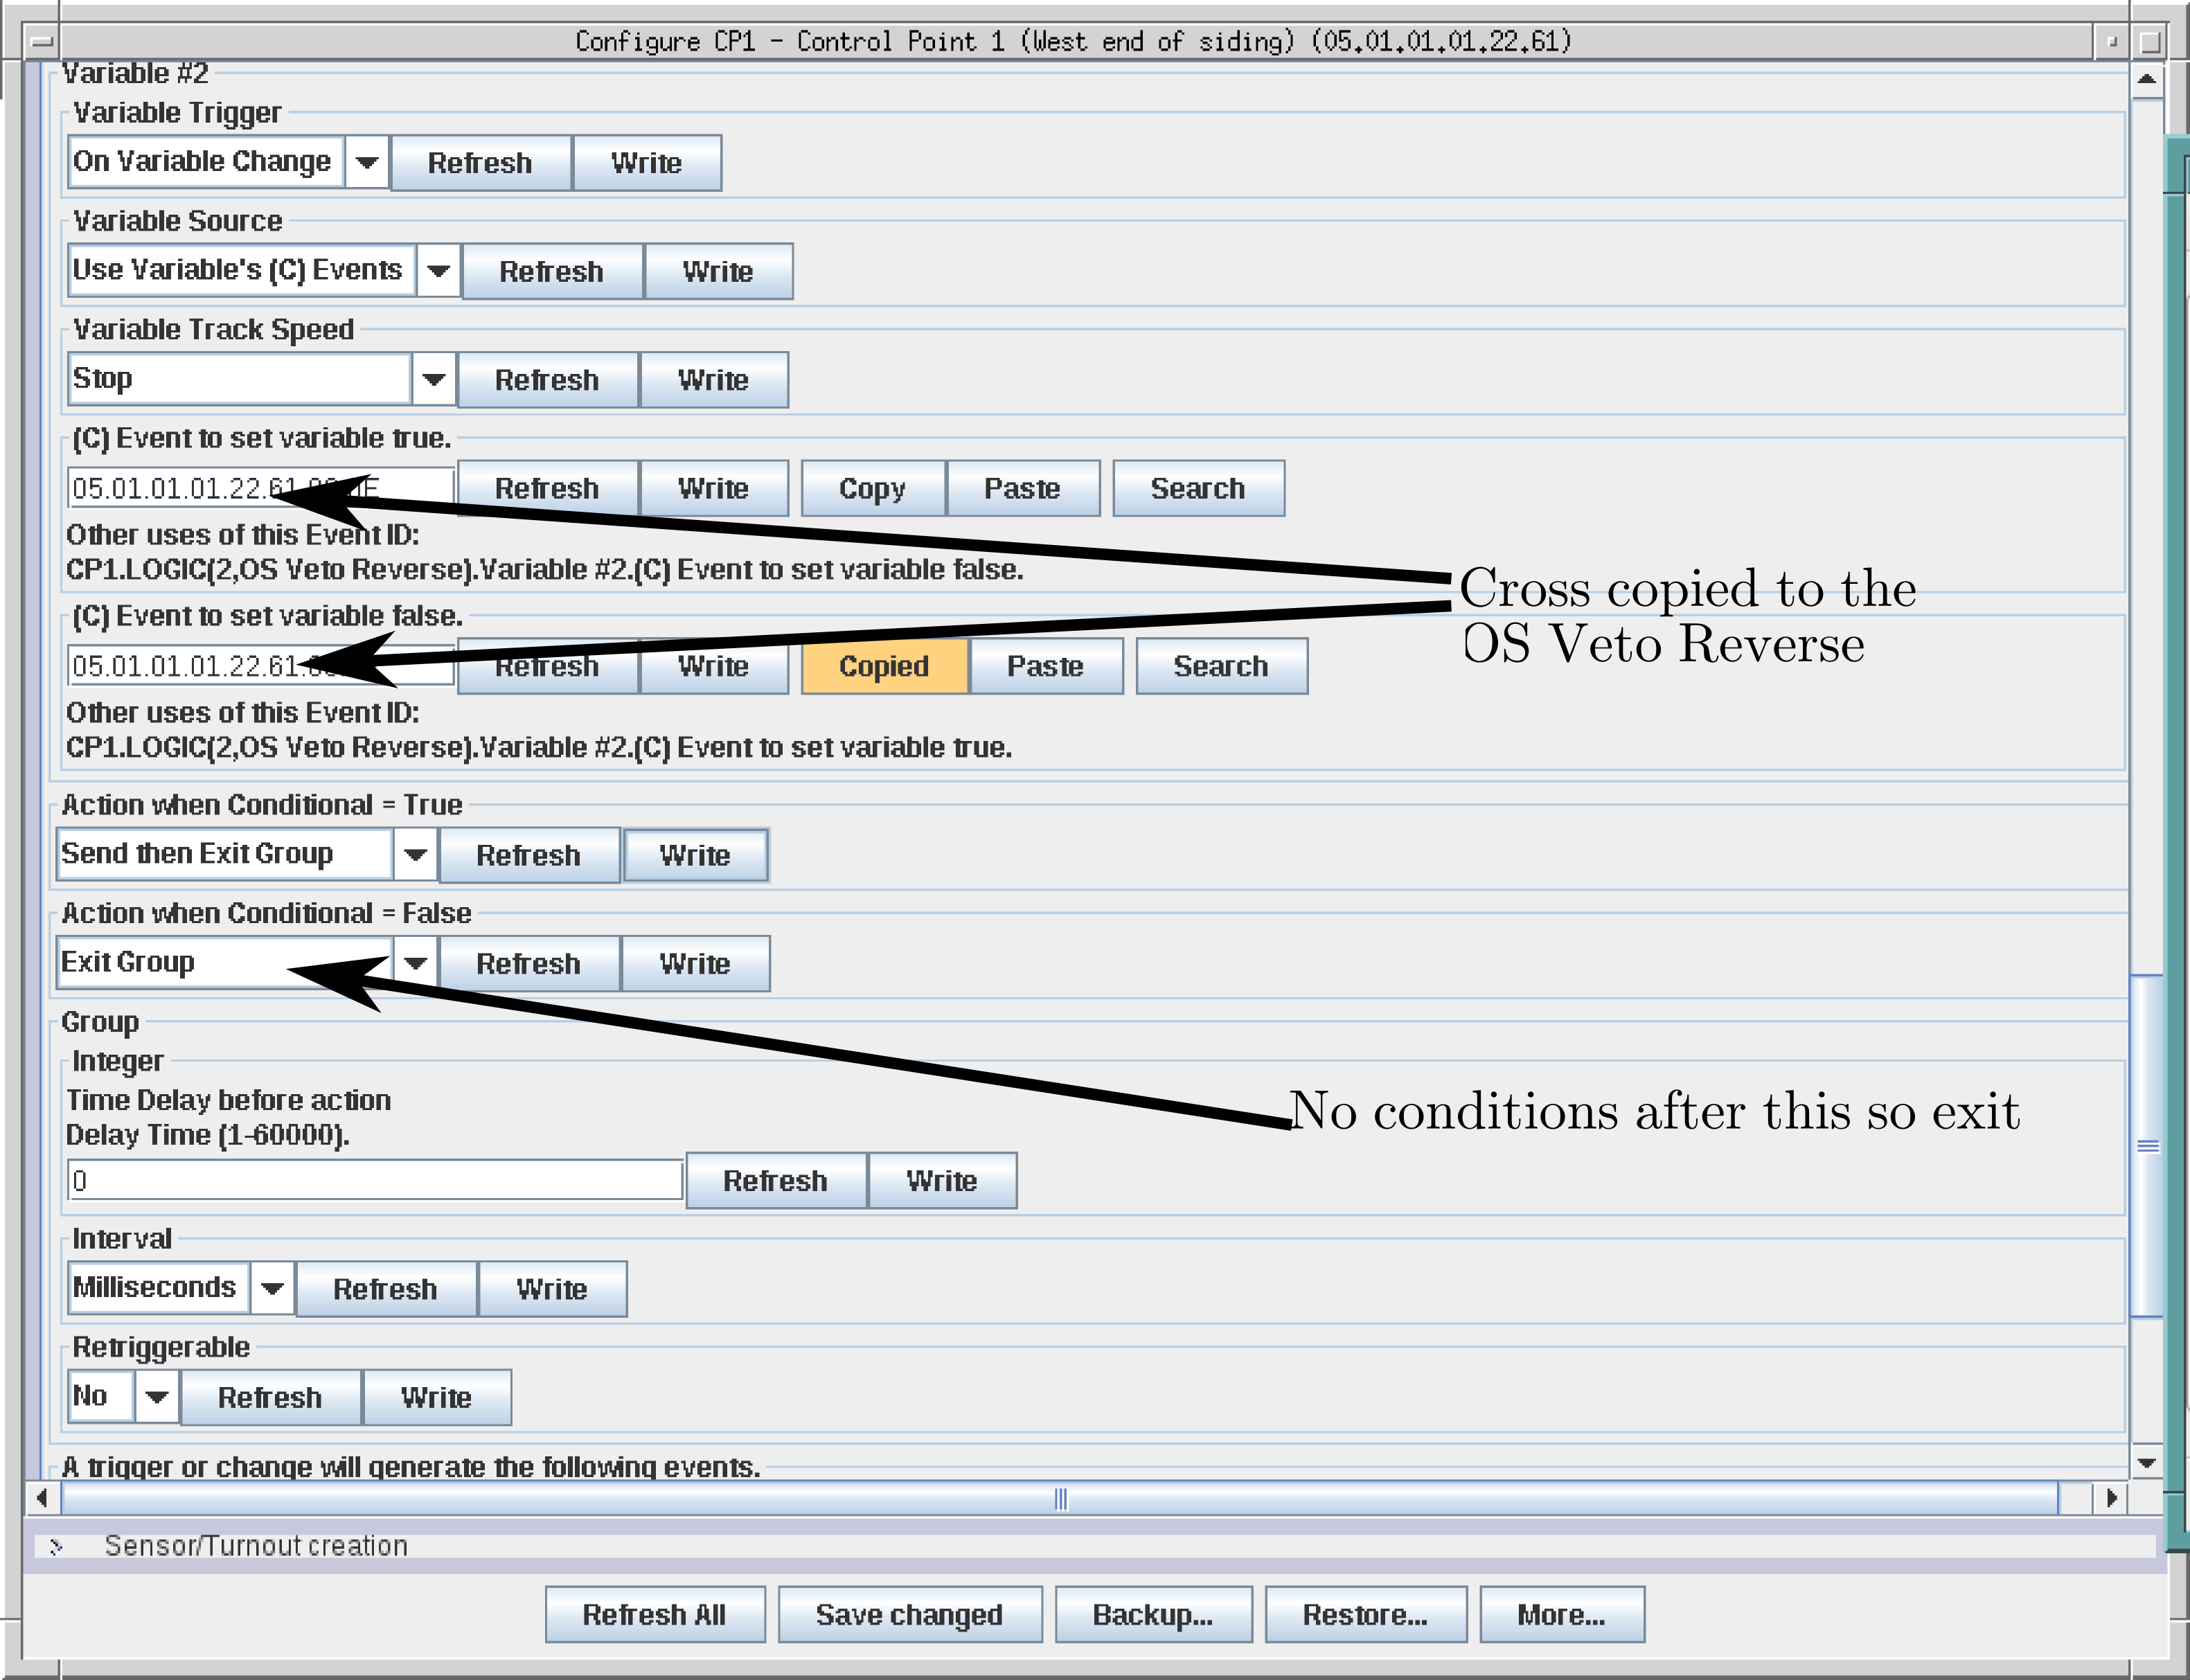
\includegraphics[width=5in]{CP1-OSVeto-Normal2-Annotated.png}
\caption{CP1 OS Veto, part 2 (variable 2)}
\label{fig:CP1-OSVeto-Normal2}
\end{centering}\end{figure}                                                    
\begin{figure}[hbpt]\begin{centering}%                                         
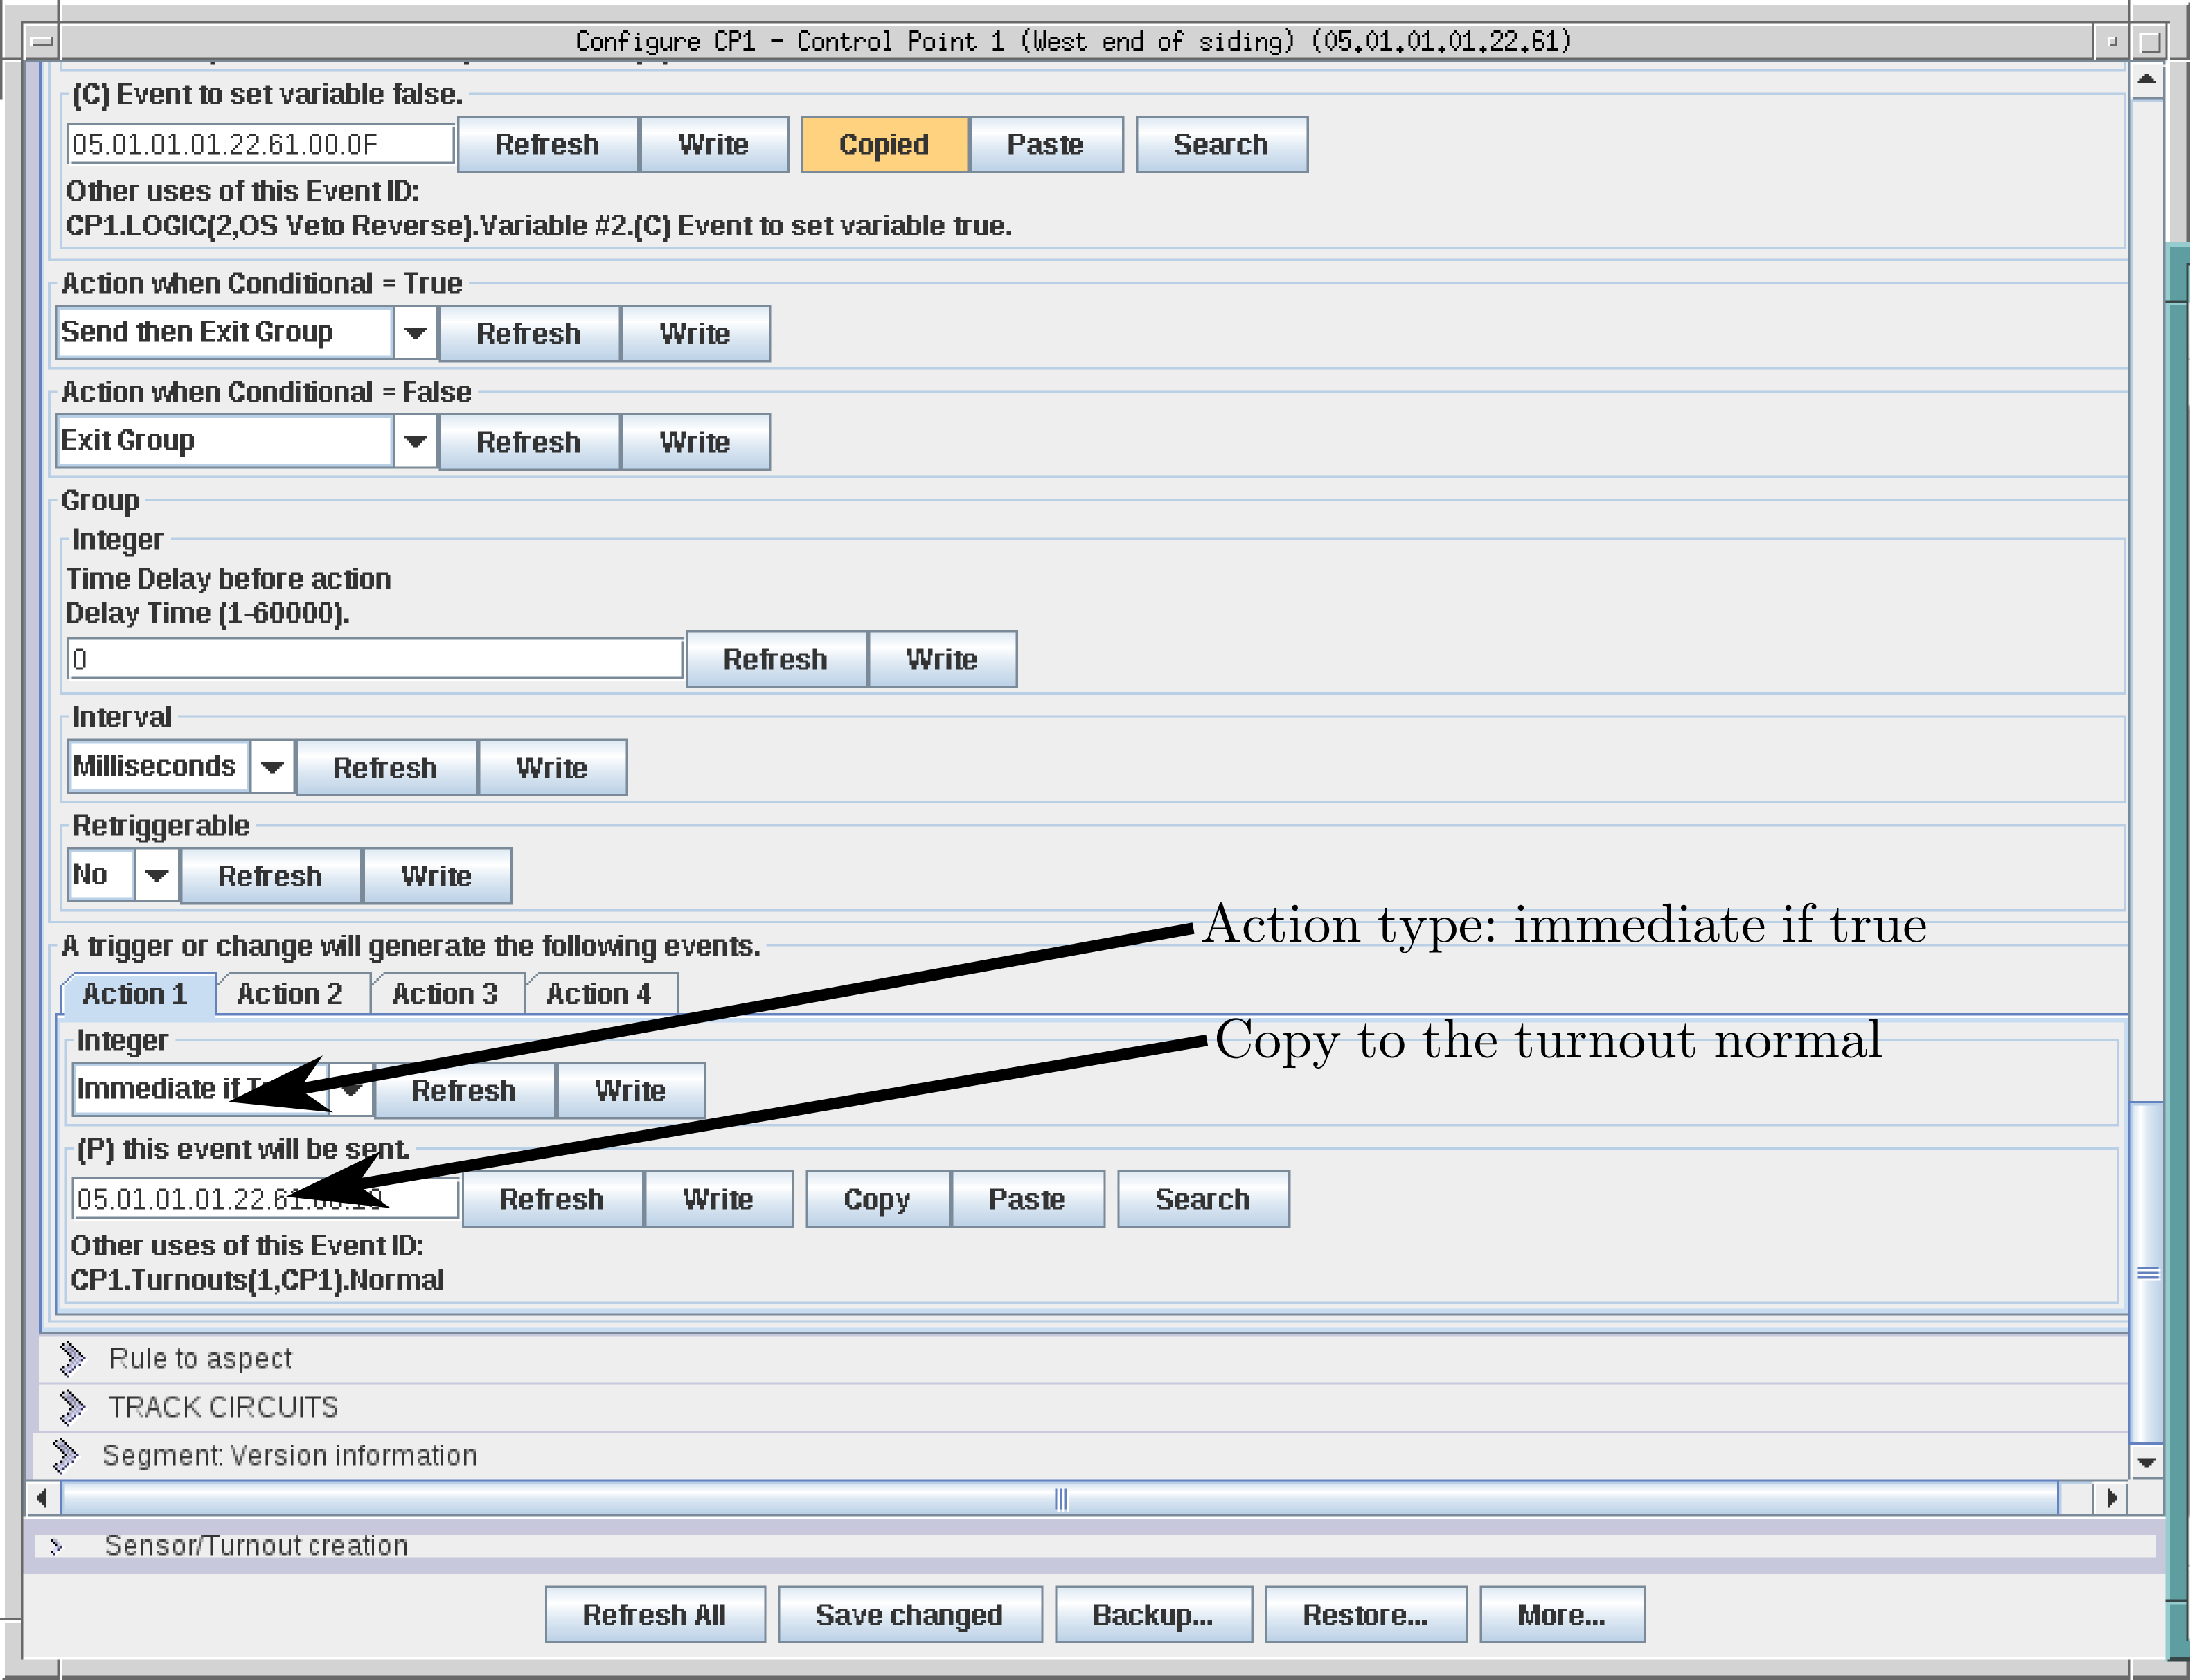
\includegraphics[width=5in]{CP1-OSVeto-Normal3-Annotated.png}
\caption{CP1 OS Veto, part 3 (Action 1)}
\label{fig:CP1-OSVeto-Normal3}
\end{centering}\end{figure}                                                    
Next we use the CP1 OS occupancy detector as a veto to prevent moving the 
points while a train is occupying the turnout.  This is done with two logic 
elements.  One logic handles the normal request and the other handles the 
reverse request.  The second variable consumer events for these logics become 
the external events consumed for throwing the turnout and the variable 2 
events for the first logic are cross copied to the second logic.

\clearpage
\subparagraph{Logic for signal CP1ME}
This signal uses a chain of four logic blocks to implement this logic:
\begin{verbatim}
if OS is occupied then
    show Stop
else if CP1 points aligned for the siding then
    show Take Siding
else if Main line beyond the turnout is occupied then
    show Approach
else
    show Clear
\end{verbatim}

\begin{figure}[hbpt]\begin{centering}%
\includegraphics[width=5in]{CP1ME-Stop-Logic-Config1.png}
\caption{Configuring the logic element for CP1ME Stop aspect, part 1}
\label{fig:CP1ME-Stop-Logic-Config1}
\end{centering}\end{figure}
\begin{figure}[hbpt]\begin{centering}%
\includegraphics[width=5in]{CP1ME-Stop-Logic-Config2.png}
\caption{Configuring the logic element for CP1ME Stop aspect, part 2}
\label{fig:CP1ME-Stop-Logic-Config2}
\end{centering}\end{figure}
\begin{figure}[hbpt]\begin{centering}%
\includegraphics[width=5in]{CP1ME-Stop-Logic-Config3.png}
\caption{Configuring the logic element for CP1ME Stop aspect, part 3}
\label{fig:CP1ME-Stop-Logic-Config3}
\end{centering}\end{figure}
First we configure the logic element for the Stop aspect (the most restrictive 
aspect) of signal CP1ME, as shown in Figures 
\ref{fig:CP1ME-Stop-Logic-Config1}, \ref{fig:CP1ME-Stop-Logic-Config2}, and 
\ref{fig:CP1ME-Stop-Logic-Config3}.

\clearpage
\begin{figure}[hbpt]\begin{centering}%
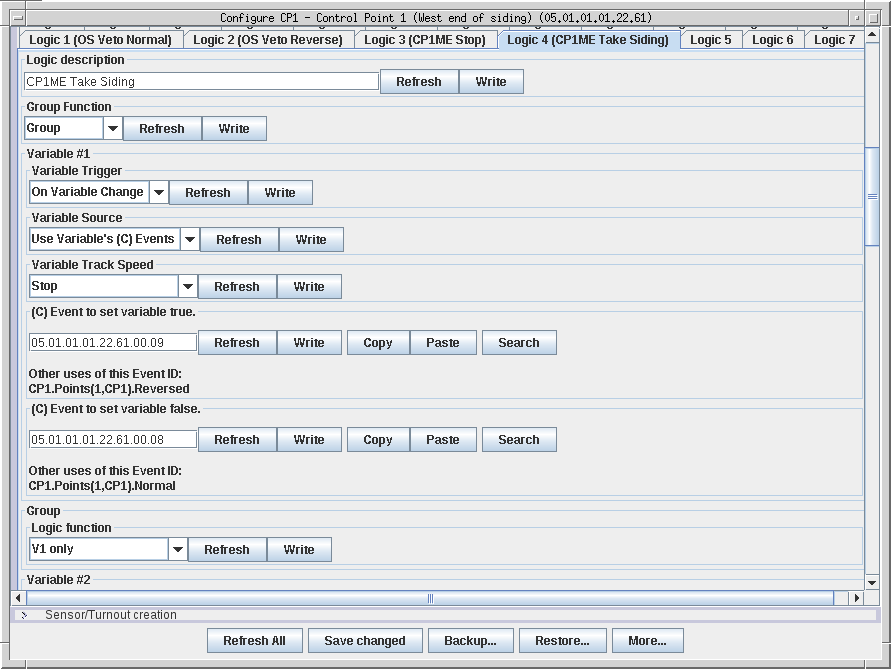
\includegraphics[width=5in]{CP1ME-TakeSiding-Logic-Config1.png}
\caption{Configuring the logic element for CP1ME Take Siding aspect, part 1}
\label{fig:CP1ME-TakeSiding-Logic-Config1}
\end{centering}\end{figure}
\begin{figure}[hbpt]\begin{centering}%
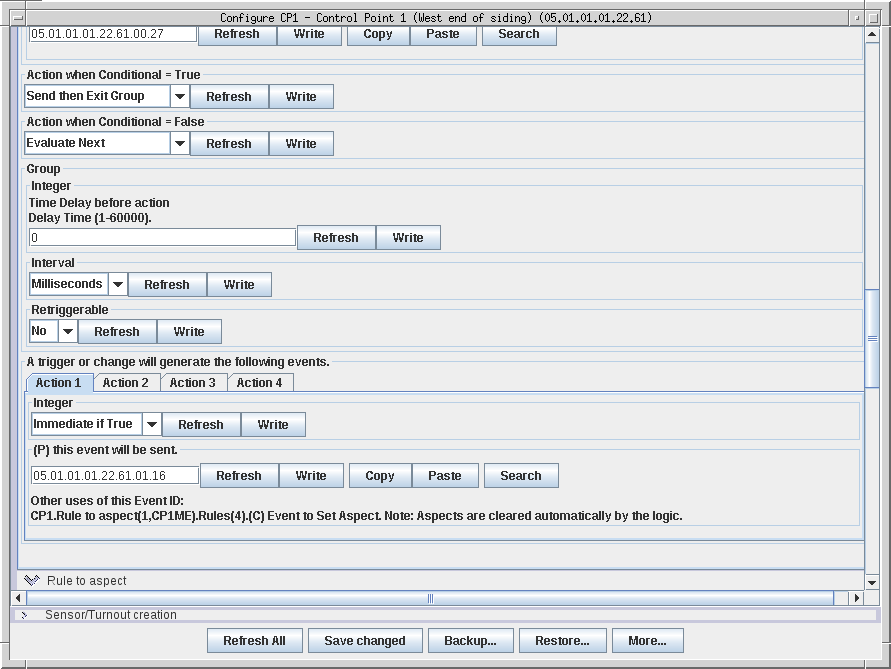
\includegraphics[width=5in]{CP1ME-TakeSiding-Logic-Config2.png}
\caption{Configuring the logic element for CP1ME Take Siding aspect, part 2}
\label{fig:CP1ME-TakeSiding-Logic-Config2}
\end{centering}\end{figure}
Next we configure the logic element for the Take Siding aspect (the next 
restrictive aspect) of signal CP1ME, as shown in Figures 
\ref{fig:CP1ME-TakeSiding-Logic-Config1} and 
\ref{fig:CP1ME-TakeSiding-Logic-Config2}.
 
\clearpage
\begin{figure}[hbpt]\begin{centering}%
\includegraphics[width=5in]{CP1ME-Approach-Logic-Config1.png}
\caption{Configuring the logic element for CP1ME Approach aspect, part 1}
\label{fig:CP1ME-Approach-Logic-Config1}
\end{centering}\end{figure}
\begin{figure}[hbpt]\begin{centering}%
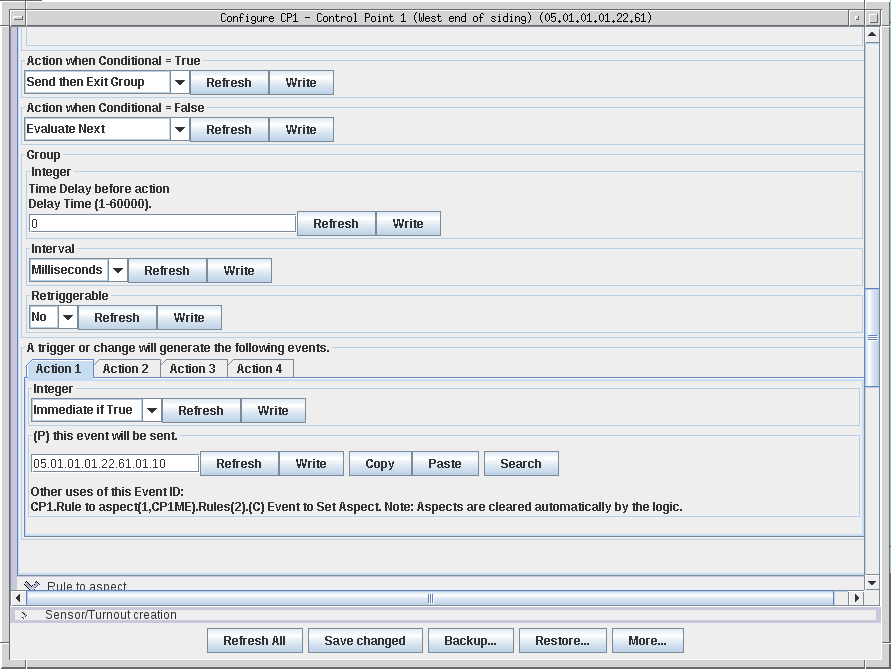
\includegraphics[width=5in]{CP1ME-Approach-Logic-Config2.png}
\caption{Configuring the logic element for CP1ME Approach aspect, part 2}
\label{fig:CP1ME-Approach-Logic-Config2}
\end{centering}\end{figure}
Next we configure the logic element for the Approach aspect (the next 
restrictive aspect) of signal CP1ME, as shown in Figures 
\ref{fig:CP1ME-Approach-Logic-Config1} and 
\ref{fig:CP1ME-Approach-Logic-Config2}. We have not set up the events for the 
variable yet, since these events will come from the other ESP32-PWMHalfSiding 
board's second occupancy detector, which is for the main line between the 
sidings.

\clearpage
\begin{figure}[hbpt]\begin{centering}%
\includegraphics[width=5in]{CP1ME-Clear-Logic-Config1.png}
\caption{Configuring the logic element for CP1ME Clear aspect, part 1}
\label{fig:CP1ME-Clear-Logic-Config1}
\end{centering}\end{figure}
\begin{figure}[hbpt]\begin{centering}%
\includegraphics[width=5in]{CP1ME-Clear-Logic-Config2.png}
\caption{Configuring the logic element for CP1ME Clear aspect, part 2}
\label{fig:CP1ME-Clear-Logic-Config2}
\end{centering}\end{figure}
Lastly we configure the logic element for the Clear aspect (the least 
restrictive aspect) of signal CP1ME, as shown in Figures 
\ref{fig:CP1ME-Clear-Logic-Config1} and 
\ref{fig:CP1ME-Clear-Logic-Config2}. This is an unconditional logic and is the 
last in this chain.


 

\clearpage
\subsection{Implementing Automatic Block Signals}

\begin{figure}[hbpt]\begin{centering}%
\includegraphics[width=5in]{ABSTrack_Annotated.png}
\caption{A Bi-directional track with ABS}
\label{fig:ABSTrack}
\end{centering}\end{figure}
\begin{figure}[hbpt]\begin{centering}%
\includegraphics[width=5in]{ABSTrack_Wiring.png}
\caption{Wiring two Bi-directional ABS blocks}
\label{fig:ABSTrack_Wiring}
\end{centering}\end{figure}
A stretch of Bi-directional track with ABS is shown in 
Figure~\ref{fig:ABSTrack} and Figure~\ref{fig:ABSTrack_Wiring} shows how two 
of the blocks would be wired to a ESP32 HalfSiding board. Additional boards 
would be used for additional pairs of blocks.


\clearpage
\subsection{Crossing with Interchange}


